%!TEX program = xelatex
\documentclass[twoside,a4paper]{article}
\usepackage[english]{babel}
\usepackage{amsmath,amsfonts,amssymb,amsthm,bbm,mathrsfs}
\usepackage{hyperref}
\usepackage{listings}
\usepackage{graphicx}
\usepackage{svg}
\usepackage{pgf,tikz,pgfplots}
\usetikzlibrary{arrows}
\pgfplotsset{compat=1.16}

\theoremstyle{plain}
\newtheorem{theorem}{Theorem}[section]
\newtheorem{proposition}[theorem]{Proposition}
\newtheorem{lemma}[theorem]{Lemma}
\newtheorem{corollary}[theorem]{Corollary}
\newtheorem{property}[theorem]{Property}
\newtheorem{properties}[theorem]{Properties}
\newtheorem{conjecture}[theorem]{Conjecture}

\theoremstyle{definition}
\newtheorem{exercise}[theorem]{Exercise}
\newtheorem{definition}[theorem]{Definition}
\newtheorem{example}[theorem]{Example}

\theoremstyle{remark}
\newtheorem{remark}[theorem]{Remark}
\newtheorem{fact}[theorem]{Fact}

\numberwithin{equation}{section}

\hypersetup{%
  colorlinks = true
}

\makeatletter
\def\maxwidth{ %
  \ifdim\Gin@nat@width>\linewidth
    \linewidth
  \else
    \Gin@nat@width
  \fi
}
\makeatother

\definecolor{fgcolor}{rgb}{0.345, 0.345, 0.345}
\newcommand{\hlnum}[1]{\textcolor[rgb]{0.686,0.059,0.569}{#1}}%
\newcommand{\hlstr}[1]{\textcolor[rgb]{0.192,0.494,0.8}{#1}}%
\newcommand{\hlcom}[1]{\textcolor[rgb]{0.678,0.584,0.686}{\textit{#1}}}%
\newcommand{\hlopt}[1]{\textcolor[rgb]{0,0,0}{#1}}%
\newcommand{\hlstd}[1]{\textcolor[rgb]{0.345,0.345,0.345}{#1}}%
\newcommand{\hlkwa}[1]{\textcolor[rgb]{0.161,0.373,0.58}{\textbf{#1}}}%
\newcommand{\hlkwb}[1]{\textcolor[rgb]{0.69,0.353,0.396}{#1}}%
\newcommand{\hlkwc}[1]{\textcolor[rgb]{0.333,0.667,0.333}{#1}}%
\newcommand{\hlkwd}[1]{\textcolor[rgb]{0.737,0.353,0.396}{\textbf{#1}}}%
\let\hlipl\hlkwb

\usepackage{framed}
\makeatletter
\newenvironment{kframe}{%
 \def\at@end@of@kframe{}%
 \ifinner\ifhmode%
  \def\at@end@of@kframe{\end{minipage}}%
  \begin{minipage}{\columnwidth}%
 \fi\fi%
 \def\FrameCommand##1{\hskip\@totalleftmargin \hskip-\fboxsep
 \colorbox{shadecolor}{##1}\hskip-\fboxsep
     % There is no \\@totalrightmargin, so:
     \hskip-\linewidth \hskip-\@totalleftmargin \hskip\columnwidth}%
 \MakeFramed {\advance\hsize-\width
   \@totalleftmargin\z@ \linewidth\hsize
   \@setminipage}}%
 {\par\unskip\endMakeFramed%
 \at@end@of@kframe}
\makeatother

\definecolor{shadecolor}{rgb}{.97, .97, .97}
\definecolor{messagecolor}{rgb}{0, 0, 0}
\definecolor{warningcolor}{rgb}{1, 0, 1}
\definecolor{errorcolor}{rgb}{1, 0, 0}
\newenvironment{knitrout}{}{} % an empty environment to be redefined in TeX

\usepackage{alltt}
\usepackage{upquote}

%Afkortingen voor wiskundige symbolen
\newcommand{\N}{\mathbb{N}}
\newcommand{\Z}{\mathbb{Z}}
\newcommand{\Q}{\mathbb{Q}}
\newcommand{\R}{\mathbb{R}}
\renewcommand{\C}{\mathbb{C}}

\let\P\relax
\DeclareMathOperator{\P}{\mathbb{P}}
\DeclareMathOperator{\V}{\mathbb{V}}
\DeclareMathOperator{\E}{\mathbb{E}}
\DeclareMathOperator{\1}{\mathbbm{1}}
\newcommand{\F}{\mathcal{F}}
\renewcommand{\G}{\mathcal{G}}
\renewcommand{\H}{\mathcal{H}}
\newcommand{\B}{\mathcal{B}}
\newcommand{\X}{\mathcal{X}}
\newcommand{\Y}{\mathcal{Y}}

\DeclareMathOperator{\supp}{supp}
\DeclareMathOperator{\range}{range}

\newcommand{\Pmod}{\mathcal{P}^*}
\newcommand{\Psafe}{\tilde{\P}}
\newcommand{\Uonesafe}{\tilde{\1}_U}
\newcommand{\Usafe}{\tilde{U}}

\newcommand{\EnvIndSafe}{\1_{\{B=2A\}}}
\newcommand{\DieInd}{\1_{\{Y=3\}}}
\newcommand{\DieIndSafe}{\tilde{\1}_{\{Y=3\}}}
\newcommand{\ChildInd}{\1_{\{U=bg\}}}
\newcommand{\ChildIndSafe}{\tilde{\1}_{\{U=bg\}}}
\newcommand{\ChildTwoInd}{\1_{\{U=bb\}}}
\newcommand{\ChildTwoIndSafe}{\tilde{\1}_{\{U=bb\}}}
\newcommand{\GeneralInd}{\1_{\{U=u'\}}}
\newcommand{\GeneralGenInd}{\1_{\{U\in\Y'\}}}
\newcommand{\GeneralGenIndSafe}{\tilde{\1}_{\{U\in\Y'\}}}

\title{Safe probabilities}
\author{Mathijs Kolkhuis Tanke}
\date{\today}

\begin{document}
\maketitle

\begin{abstract}
Conditioning probabilities is one of the fundamental aspects of probability theory, yet results can become counter-intuitive. One example is the Monty~Hall's three door problem, where there is a vast debate which strategy the user should take. Peter Grünwald \cite{Grunwald16} formalized probability distributions in order to make reliable predictions on partial domains. We apply this reformalization on various known paradoxes, such as Monty~Hall's problem and the two envelope problem.
\end{abstract}

\tableofcontents


\section{Discrete safe probabilities}
This whole section is taken from \cite{Grunwald16}. Here we'll define discrete safe probabilities and state some relevant properties and theorems. All random variables in this section are discrete.

First we need to define range and support. The \emph{range} of a random variable $S:\X\to\Y$ is
\[\range(S):=\{s\in\Y|s=S(x),x\in\X\}.\]
The \emph{support} of $S$ under distribution $\P$ is
\[\supp_{\P}(S):=\{s\in\Y|\P(S=s)>0\}.\]
For any random variables $U$ and $V$ on $\X$ we write $U\rightsquigarrow V$ if there is a function $f$ such that $f(U)=V$. If function $f$ is known, we write $U\stackrel{f}{\rightsquigarrow}V$.
\begin{definition}[Safe probabilities]\label{def:safeprop}
Let $\Omega$ be an outcome space and let $\Pmod$ be a set of distributions on $\Omega$. Let $U$ be a real-valued random variable and let $V$ be a random variable on $\Omega$. Let $\Psafe$ be a probability distribution on $\Omega$. Then $\Psafe$ is \emph{safe} for
\begin{itemize}
	\item $\langle U\rangle|\langle V\rangle$ if $\E_{\P}[U]=\E_{\P}[\E_{\Psafe}[U|V]]$ holds for all $\P\in\Pmod$. This $\Psafe$ is called \emph{unbiased} for $U|V$.
	\item $\langle U\rangle|[V]$ if $E_{\P}[U]=\E_{\Psafe}[U|V=v]$ holds for all $v\in\supp_{\Psafe}(V)$. This $\Psafe$ is called \emph{marginally valid} for $U|V$. 
\end{itemize}
\end{definition}
\begin{definition}[Stronger safety]\label{def:strongsafeprop}
Let $\Omega,\Pmod,U,V$ and $\Psafe$ as above. Then $\Psafe$ is \emph{safe} for
\begin{itemize}
	\item $U|\langle V\rangle$ if for all random variables $U'$ on $\Omega$ with $U\rightsquigarrow U'$ distribution $\Psafe$ is safe for $\langle U'\rangle|\langle V\rangle$.
	\item $U|[V]$ if for all random variables $U'$ on $\Omega$ with $U\rightsquigarrow U'$ distribution $\Psafe$ is safe for $\langle U'\rangle|[V]$.
\end{itemize}
\end{definition}
\begin{proposition}\label{prop:safeimply}
If $\Psafe$ is safe for $\langle U\rangle|[V]$, it is also safe for $\langle U\rangle|\langle V\rangle$. If $\Psafe$ is safe for $U|[V]$, it is also safe for $U|\langle V\rangle$.
\end{proposition}
\begin{proposition}[Basic interpretations of safety]\label{prop:safeproperties}
Consider the setting above. Then
\begin{enumerate}
	\item $\Psafe$ is safe for $U|\langle V\rangle$ if and only if for all $\P\in\Pmod$ there is a distribution $\P'$ on $\Omega$ with $\P'[U=u,V=v]=\Psafe[U=u|V=v]\P[V=v]$ for all $(u,v)\in\range((U,V))$ such that $\P'[U]=\P[U]$.
	\item $\Psafe$ is safe for $\langle U\rangle|V$ if and only if \[\E_{\P}[U|V]=\E_{\Psafe}[U|V]\] holds with probability $1$ for all $\P\in\Pmod$. This $\Psafe$ is called \emph{squared error-optimal} for $U|V$.
	\item $\Psafe$ is safe for $U|V$ if and only if \[\P[U|V]=\Psafe[U|V]\] holds with probability $1$ for all $\P\in\Pmod$. This $\Psafe$ is called \emph{valid} for $U|V$.
	\item $\Psafe$ is safe for $U|[V]$ if and only if $\P[U]=\Psafe[U|V=v]$ for all $\P\in\Pmod$ and $v\in\supp_{\Psafe}(V)$.
\end{enumerate}
\end{proposition}
\begin{definition}[Discrete pivot]\label{def:discpivot}
Let $U,V$ as before. Assume $\Omega$ is countable. A random variable $U'$ is a \emph{discrete pivot} for $U|V$ if
\begin{enumerate}
	\item $(U,V)\rightsquigarrow U'$ holds, thus there is a function $f$ with $U'=f(U,V)$.
	\item For each fixed $v\in\range(V)$ the function
	\[f_v\colon\range(U|V=v)\to\range(U'),\qquad u\mapsto f(u,v)\] is injective.
	\item All $\P\in\Pmod$ agree on $U'$, thus for all $\P_1,\P_2\in\Pmod$ we have $\P_1(U')=\P_2(U')$.
\end{enumerate}
Pivot $U'$ is \emph{simple} if $f_v$ is a bijection for all $v\in\range(V)$.
\end{definition}
\begin{definition}[Continuous pivot]\label{def:contpivot}
Let $U,V$ as before. Assume that $\range(U|V=v)$ is a possibly unbounded interval for all $v\in\range(V)$. A random variable $U'$ is a \emph{continuous pivot} for $U|V$ if
\begin{enumerate}
	\item $(U,V)\rightsquigarrow U'$ holds, thus there is a function $f$ with $U'=f(U,V)$.
	\item For each fixed $v\in\range(V)$ the function
	\[f_v\colon\range(U|V=v)\to\range(U'),\qquad u\mapsto f(u,v)\] is injective, continuous and uniformly monotonic.
	\item All $\P\in\Pmod$ agree on $U'$, thus for all $\P_1,\P_2\in\Pmod$ we have $\P_1(U')=\P_2(U')$. Furthermore, for all $\P\in\Pmod$ the range $\range(U')$ must be a possibly unbounded interval and there must be a density $f$ with $f(u)>0$ for all $u$ in the interior of $\range(U')$.
\end{enumerate}
Pivot $U'$ is \emph{simple} if $f_v$ is a bijection for all $v\in\range(V)$.
\end{definition}
\begin{definition}[Pivotal safety]\label{def:pivotsafe}
Let $U,V$ as before and let $\Psafe$ be an arbitrary distribution on $\Omega$. If $V$ has full support under $\Psafe$ and $U'$ is a discrete pivot for $\Psafe$ such that $\Psafe$ is safe for $U'|[V]$, then $\Psafe$ is \emph{pivotally safe} for $U|V$ with pivot $U'$.
\end{definition}
For two random variables $U,V$, let $\tilde{p}_{[U|V]}(U|V)$ be the random variable mapping $x\in\X$ to $\tilde{p}_{[U|V]}(U|V)(x)=\Psafe(U=U(x)|V=V(x))$.
\begin{theorem}[Grünwald (2018)]\label{thm:pivotsafe}
Let $\Omega$ be countable, $U$ a real-valued random variable and $V$ a random variable. Suppose that for all $v\in\range(V)$ there are no two $u_1,u_2\in\range(U|V=v)$ such that $\Psafe(U=u_1|V=v)=\Psafe(U=u_2|V=v)$. Then the following statements are equivalent:
\begin{enumerate}
	\item $\Psafe$ is safe for $\tilde{p}(U|V)|[V]$.
	\item $\Psafe$ is pivotally safe for $U|V$ with simple pivot $U'=\tilde{p}(U|V)$.
	\item $\Psafe$ is pivotally safe for $U|V$ for some simple pivot $U''$.
\end{enumerate}
\end{theorem}
\section{Monty~Hall's three door problem}
Take a look at Monty~Hall's three door problem. There are three doors called $1$, $2$ and $3$. The player initially chooses door~1. Then either doors $2$ or $3$ are opened by the game master, however if a door has a car, it cannot be opened.\\
Let $U\in\{1,2,3\}$ be the random variable denoting which door has a car and let $V\in\{2,3\}$ be the random variable of the game master opening doors. The probability space is 
\[\Omega=\left\{(1,2),(1,3),(2,3),(3,2)\right\}\]
having all possible of combinations and opened doors. Suppose door~2 is opened. The player wants to know what $\P[U=1|V=2]$ is. If $\P[U=1|V=2]<\frac{1}{2}$ for example holds, the player must switch for higher changes of obtaining the car. However, the player does not know which distribution on $\Omega$ is taken here.

\subsection{Multiple priors}\label{sec:monty_multiprior}
One strategy is to use multiple priors to fully model the problem. Suppose $\P[V=2|U=1]=p$, thus the game master opens door~2 with probability $p$ is the car is behind door~1. Suppose further that $\P[U=u]=q_u$ with $q_1+q_2+q_3=1$, modelling the distribution of the car between the three doors. In this case we have
\begin{align*}
\P[U=1|V=2]&=\frac{\P[U=1,V=2]}{\P[V=2]}=\frac{\P[V=2|U=1]\P[U=1]}{\sum_{u\in\{1,3\}}\P[V=2|U=u]\P[U=u]}\\
&=\frac{pq_1}{pq_1+q_3},\\
\P[U=1|V=3]&=\frac{(1-p)q_1}{q_1+(1-p)q_3}.
\end{align*}
If $U$ is distributed uniformly, we have $\P[U=1|V=2]\in\left[0,\frac{1}{2}\right]$. Without any information, the probabilities can take any value from $0$ to $1$. Therefore without watching many previous shows of Monty~Hall and calculating the experimental frequencies, this method does not provide much insight in the full risk of switching. What must be noted, is that $\P[U=1|V=v]$ is capped by $\frac{1}{2}$ for both $v\in\{2,3\}$, thus one could argue that switching is always advised.

\subsection{Using safe probabilities}
Let us now consider the three doors problem from the viewpoint of safe probabilities. We will take a look at example~11 from \cite{Grunwald16} as it states which safe probabilities are advised to be used. \cite{Grunwald16} as an extension of \cite{Grunwald18} and example~11 from \cite{Grunwald16} is not yet published. Therefore we will prove all statements from this example~11 when we use them.

First we need a model of probabilities. We can take as model all possible probability distributions on $\Omega$, however this will vastly overfit our search to a safe probability. A reasonable assumption to make is that the car is distributed evenly between the doors, thus $U$ takes on the uniform distribution. Therefore take
\[\Pmod=\left\{\P\text{ on }\Omega\middle|\forall u\in\{1,2,3\}:\P[U=u]=\frac{1}{3}\right\}.\]
This model is reasonable to use, as when contestants note that Monty~Hall favours one door above the other two, they will always choose that door. Thus it is in Monty~Hall's best interest to never favour one door when initially placing the car.

\subsubsection{Pivotal safety}
Now we will find a distribution $\Psafe$ that is pivotally safe for $U|V$, as is done in example~11 of \cite{Grunwald18}, with pivot $\1_{\{U=1\}}$. We first need to prove that $\1_{\{U=1\}}$ indeed is a pivot.

\begin{lemma}
The random variable $U'=\1_{\{U=1\}}$ is a simple pivot for $U|V$.
\end{lemma}
\begin{proof}
The proof is nothing more than checking the three requirements of definition~\ref{def:discpivot}.
\begin{enumerate}
	\item Take as function $f(U,V)=\1_{\{U=1\}}$. This is a well-defined function, therefore $(U,V)\rightsquigarrow U'$.
	\item Note that $\range(V)=\{2,3\}$. Take $v=2$, then $\range(U|V=2)=\{1,3\}$. We have $f_2(1)=f(1,2)=1$ and $f_2(3)=f(3,2)=0$, thus $f_2$ is a bijection. Taking $v=3$ we get $f_3(1)=1$ and $f_3(2)=0$, thus $f_3$ is a bijection as well.
	\item Take $\P_1,\P_2\in\Pmod$ arbitrarily. Note that $\range(U')=\{0,1\}$. Therefore
	\begin{align*}
		\P_1[U'=0]&=\P_1[U\in\{2,3\}]=\frac{2}{3}=\P_2[U\in\{2,3\}]=\P_2[U'=0],\\
		\P_1[U'=1]&=\P_1[U=1]=\frac{1}{3}=\P_2[U=1]=\P_2[U'=1],
	\end{align*}
	thus we have $\P_1[U']=\P_2[U']$.
\end{enumerate}
Since we have proven that $f_v$ is a bijection for all $v\in \range(V)$, the pivot $U'=\1_{\{U=1\}}$ is a simple pivot for $U|V$.
\end{proof}

Now we have a pivot we can find a distribution $\Psafe$ which is pivotally safe for $U|V$ with pivot $\1_{\{U=1\}}$. Our model already assumes that the car is initially distributed uniformly, thus the only parameter we have not modelled yet is which strategy Monty~Hall uses to open a door given the car is behind door~1. Assume that when the car is behind door~1, it is reasonable to assume that Monty~Hall opens doors $2$ or $3$ with equal chance. Thus let $\Psafe\in\Pmod$ be defined by \[\Psafe[V=2|U=1]=\Psafe[V=3|U=1]=\frac{1}{2},\]
the uniform distribution on $V|U=1$. Now Bayes can be used to calculate $U|V=2$ and $U|V=3$ under $\Psafe$:
\begin{align*}
\Psafe[U=1|V=2]&=\frac{\Psafe[U=1,V=2]}{\Psafe[V=2]}=\frac{\Psafe[V=2|U=1]\Psafe[U=1]}{\sum_{u\in\{1,3\}}\Psafe[V=2|U=u]\P[U=u]}\\
&=\frac{\frac{1}{2}\cdot\frac{1}{3}}{\frac{1}{2}\cdot\frac{1}{3}+1\cdot\frac{1}{3}}=\frac{1}{3}.
\end{align*}
Using the same calculation one can show that $\Psafe[U=1|V=3]=\frac{1}{3}$ as well.
\begin{proposition}\label{prop:montyhallsafe1U}
The distribution $\Psafe\in\Pmod$ with uniform distribution on ${V|U=1}$ is pivotally safe for $U|V$ with pivot $U'=\1_{\{U=1\}}$.
\end{proposition}
\begin{proof}
The proof is a check of definition~\ref{def:pivotsafe}. Since \[\Psafe[V=2|U=1]=\Psafe[V=3|U=1]=\frac{1}{2},\] $V$ has full support under $\Psafe$. What only remains is checking whether $\Psafe$ is safe for $\1_{\{U=1\}}|[V]$. Proposition~\ref{prop:safeproperties} states that $\P[U']=\Psafe[U'|V=v]$ must hold for all $\P\in\Pmod$ and $v\in\supp_{\Psafe}(V)$. Take now $\P\in\Pmod$ arbitrarily. Then
	\begin{align*}
		\P[U'=0]&=\P[U\in\{2,3\}]=\frac{2}{3}=1-\Psafe[U'=1|V=2]=\Psafe[U'=0|V=2],\\
		\P[U'=1]&=\P[U=1]=\frac{1}{3}=\Psafe[U'=1|V=2],
	\end{align*}
thus $\P[U']=\Psafe[U'|V=2]$ holds. Without loss of generality $\P[U']=\Psafe[U'|V=3]$ holds as well. Therefore $\Psafe$ is safe for $U'|[V]$.

This proves that $\Psafe$ is safe for $\1_{\{U=1\}}|[V]$ and thus is pivotally safe for $U|V$ with pivot $\1_{\{U=1\}}$.
\end{proof}

Consider the random variable
\[\tilde{p}(U|V)=\begin{cases}
(1,2)\mapsto\frac{1}{3}\\
(1,3)\mapsto\frac{1}{3}\\
(2,3)\mapsto\frac{2}{3}\\
(3,2)\mapsto\frac{2}{3}
\end{cases}.\]
Since $\Psafe[U=1|V=2]\neq\P[U=3|V=2]$ and $\Psafe[U=1|V=3]\neq\Psafe[U=3|V=2]$, theorem~\ref{thm:pivotsafe} states that $\Psafe$ is safe for $\tilde{p}(U|V)|[V]$ and pivotally safe for $U|V$ with pivot $\tilde{p}(U|V)$ as well.

The only stronger version of pivotal safety we can explore is whether $\Psafe$ is safe for $\1_{\{U=1\}}|V$. Proposition~\ref{prop:safeproperties} requires $\P\left[\1_{\{U=1\}}\middle|V\right]=\Psafe\left[\1_{\{U=1\}}|V\right]$ for all $\P\in\Pmod$. Take a $\P\in\Pmod$, then according to section~\ref{sec:monty_multiprior} we have $q_1=q_2=q_3=\frac{1}{3}$ so we get
\[\P\left[\1_{\{U=1\}}=1\middle|V=2\right]=\P[U=1|V=2]=\frac{p}{p+1}.\]
However, we have $\Psafe\left[\1_{\{U=1\}}=1\middle|V=2\right]=\frac{1}{3}$ and $\frac{1}{3}=\frac{p}{p+1}$ only holds for one specific $p=\frac{1}{2}$. As for $\P$ the value of $p$ can be anything in $[0,1]$, thus the condition $\P\left[\1_{\{U=1\}}\middle|V\right]=\Psafe\left[\1_{\{U=1\}}\middle|V\right]$ does not hold for all $\P\in\Pmod$. This also proves that there is no different $\Psafe'\in\Pmod$ such that $\Psafe'\left[\1_{\{U=1\}}\middle|V\right]=\P\left[\1_{\{U=1\}}\middle|V\right]$ does hold for all $\P\in\Pmod$, as $\Psafe'[U=1|V=2]=\frac{p}{p+1}$ must hold for all $p\in[0,1]$. Thus safety for $\1_{\{U=1\}}|V$ under $\Pmod$ is only possible after further restricting $\Pmod$, however $\Pmod$ must then be restricted to a singleton which defeats the purpose of safe probabilities.

To conclude, if the player initially chooses door~1 and assumes that the car is initially placed under uniform distribution between the three doors, switching with probability $\frac{2}{3}$ yields to an unbiased and marginally valid estimate of the actual probability of obtaining the car. 

\subsubsection{Unbiased and marginally valid safe probabilities}
Now we have found a safe probability measure for $\1_{\{U=1\}}|[V]$, which is the strongest pivotal safe probability possible in this setting. We now return to $U|V$ and want to know whether we can construct a safe probability $\Psafe$ for $U|[V]$. This construction is however not possible as will be proven in the following proposition.

\begin{proposition}\label{prop:montyhallsafeU}
Let $\Pmod$ be the set of distributions on $\Omega$ assuming the car is initially distributed evenly between the three doors, thus $\P[U=u]=\frac{1}{3}$ for all $u\in U$. Let $\Psafe$ be a distribution on $\Omega$ with
\[\Psafe[U=u|V=v]=\begin{cases}
	\frac{1}{2},&v=2,\\
	0,&u=1,v=3,\\
	1,&u=2,v=3.
	\end{cases}
\]
Then $\Psafe$ is the unique safe distribution for $\langle U\rangle|\langle V\rangle$ and $\langle U\rangle|[V]$.

There is no safe probability distribution for $U|\langle V\rangle$ or $U|[V]$.
\end{proposition}
\begin{proof}
We will first prove that there is a unique $\Psafe$ safe for $\langle U\rangle|\langle V\rangle$ by construction. If a safe distribution for the other three exists, by definition~\ref{def:strongsafeprop} and proposition~\ref{prop:safeimply} it must be that $\Psafe$. Testing the requirements results $\Psafe$ being safe for $\langle U\rangle|[V]$, but not for $U|\langle V\rangle$ and $U|[V]$.

Let $\Psafe$ be an arbitrary distribution on $\Omega$. According to definition~\ref{def:safeprop}, we want to have $\E_{\P}[U]=\E_{\P}\left[\E_{\Psafe}\left[U|V\right]\right]$ for all $\P\in\Pmod$. Take a $\P\in\Pmod$ arbitrary, then
\[\E_{\P}[U]=\sum_{u\in\{1,2,3\}}u\P[U=u]=\frac{1+2+3}{3}=2.\]
Note that
\begin{align*}
\E_{\Psafe}[U|V=2]&=\Psafe[U=1|V=2]+3\Psafe[U=3|V=2],\\
\E_{\Psafe}[U|V=3]&=\Psafe[U=1|V=3]+2\Psafe[U=2|V=3].
\end{align*}
Assume $\P[V=2|U=1]=q$ with $q\in[0,1]$, then we get
\begin{align*}
\P[V=2]&=\P[V=2|U=1]\P[U=1]+\P[V=2|U=3]\P[U=3]=\frac{q+1}{3},\\
\P[V=3]&=\P[V=3|U=1]\P[U=1]+\P[V=3|U=2]\P[U=2]=\frac{2-q}{3}.
\end{align*}
We are now able to compute $\E_{\P}\left[\E_{\Psafe}\left[U|V\right]\right]$:
\begin{align*}
\E_{\P}\left[\E_{\Psafe}\left[U|V\right]\right]&=\E_{\Psafe}[U|V=2]\P[V=2]+\E_{\Psafe}[U|V=3]\P[V=3]\\
&=\E_{\Psafe}[U|V=2]\frac{q+1}{3}+\E_{\Psafe}[U|V=3]\frac{2-q}{3}.
\end{align*}
Write $\Psafe[U=1|V=2]=a$ and $\Psafe[U=1|V=3]=b$ for simplicity, then the expression for $\E_{\P}\left[\E_{\Psafe}\left[U|V\right]\right]$ becomes
\begin{align*}
\E_{\P}\left[\E_{\Psafe}\left[U|V\right]\right]&=(a+3(1-a))\frac{q+1}{3}+(b+2(1-b))\frac{2-q}{3}\\
&=\frac{1}{3}\left(q(1+b-2a)-2a-2b+7\right).
\end{align*}
Since $\E_{\P}\left[\E_{\Psafe}\left[U|V\right]\right]=2$ must hold for all $q\in[0,1]$, it is immediately clear that $1+b-2a=0$ must hold. From here $7-2a-2b=6$ immediately arises, thus after rewriting we get the following system:
\[\begin{cases}
2a-b=1\\
2a+2b=1
\end{cases}\]
This system is uniquely solved by $a=\frac{1}{2}$ and $b=0$. Therefore all safe distributions $\Psafe$ for $\langle U\rangle|\langle V\rangle$ are given by
\[\Psafe[U=u|V=v]=\begin{cases}
	\frac{1}{2},&v=2,\\
	0,&u=1,v=3,\\
	1,&u=2,v=3.
	\end{cases}
\]
This $\Psafe$ has full support and range for $V$, thus $\range_{\Psafe}(V)=\supp_{\Psafe}(V)=\{2,3\}$.


Consider now safety for $\langle U\rangle|[V]$. The only possible safe distribution is $\Psafe$ by proposition~\ref{prop:safeimply}. Take $\P\in\Pmod$ arbitrary, then we can calculate that
\begin{align*}
\E_{\Psafe}[U|V=2]&=1\cdot\Psafe[U=1|V=2]+3\cdot\Psafe[U=3|V=2]=\frac{1}{2}+\frac{3}{2}=2=\E_{\P}[U],\\
\E_{\Psafe}[U|V=3]&=0\cdot\Psafe[U=1|V=3]+2\cdot\Psafe[U=2|V=3]=0+2=2=\E_{\P}[U].
\end{align*}
Thus $\Psafe$ is safe for $\langle U\rangle|[V]$.

Now assume $\Psafe$ is safe for $U|\langle V\rangle$. Suppose a $\P'$ exists fulfilling the role of $\P'$ in proposition~\ref{prop:safeproperties}. Take a $\P\in\Pmod$ and assume $\P[V=2|U=1]=q$ with $q\in[0,1]$. Consider $u=2$. We have $\Psafe[U=2|V=3]=1$ and $\P[V=3]=\frac{2-q}{3}$, therefore
\[\P'[U=2,V=3]=\Psafe[U=2|V=3]\P[V=3]=\frac{2-q}{3}.\]
As on $\Omega$ the only possibility for $V=3$ is when $U=2$, we also have \[\frac{2-q}{3}=\P'[U=2,V=3]=\P'[U=2]=\P[U=2]=\frac{1}{3}.\]
We now have a contradiction, as $2-q=1$ is not possible for all $q\in[0,1]$, thus $\Psafe$ is not safe for $U|\langle V\rangle$. As $\Psafe$ was the only possible distribution, no distribution in $\Pmod$ is safe for $U|\langle V\rangle$.

By proposition~\ref{prop:safeimply} there is also no distribution on $\Omega$ that is safe for $U|[V]$.
\end{proof}

\subsection{The optimal strategy}
We have found two strategies using safe probability, however we do not know whether there are better strategies possible. Let $U^*$ be a prediction of $U|V$, can we tune the distribution of $U^*$ such that the probability of winning a car $\P[U^*=U]$ is maximized for all strategies Monty~Hall can deploy? The following proposition states that in fact we can.

\begin{proposition}\label{prop:MontyHallOpt}
Let $U^*$ be a prediction of $U|V$ such that $\P[U^*=1|V=2]=p_2$ and $\P[U^*=1|V=3]=p_3$. Let $q\in[0,1]$ model the strategy of Monty Hall by $\P[V=2|U=1]=q$. The probability of winning a car is
\[\P[U^*=U]=\frac{q}{3}(p_2-p_3)+\frac{2-p_2}{3}.\]
The optimal strategy is $p_2=p_3=0$, then $\P[U^*=U]=\frac{2}{3}$ holds for all $q\in[0,1]$. There is no strategy such that $\P[U^*=U]>\frac{2}{3}$ holds for at least one $q$.
\end{proposition}
\begin{proof}
We want to compute $\P[U^*=U]$. Here $U^*$ and $U$ are dependent, as the location of the car $U$ influences which door is opened $V$, which in turn influences the result of $U^*$. Using Bayes' rule we get
\[\P[U^*=U]=\sum_{u\in\{1,2,3\}}\P[U^*=u|U=u]\P[U=u]=\frac{1}{3}\sum_{u\in\{1,2,3\}}\P[U^*=u|U=u].\]
Assume now that $\P[V=2|U=1]=q$ as in the proof of proposition~\ref{prop:montyhallsafeU}. Consider $u=1$, then
\begin{align*}
\P[U^*=1|U=1]&=\P[U^*=1|V=2,U=1]\P[V=2|U=1]\\
&\phantom{=}+\P[U^*=1|V=3,U=1]\P[V=3|U=1]\\
&=p_2q+p_3(1-q).
\end{align*}
Consider $u=2$, then 
\[\P[U^*=2|U=2]=\P[U^*=2|V=3,U=2]\P[V=3|U=2]=1-p_3.\]
Consider lastly $u=3$, then
\[\P[U^*=3|U=3]=\P[U^*=3|V=2,U=3]\P[V=2|U=3]=1-p_2.\]
Combining the three results gives us
\[\P[U^*=U]=\frac{1}{3}\sum_{u\in\{1,2,3\}}\P[\Usafe=u|U=u]=\frac{q}{3}(p_2-p_3)+\frac{2-p_2}{3}.\]

Filling in $p_2=p_3=0$ we get $\P[U^*=U]=\frac{2}{3}$. The probability $\P[U^*=U]$ has constant slope, thus if we want to have a $q\in[0,1]$ such that $\P[U^*=U]>\frac{2}{3}$, it must happen at $q\in\{0,1\}$.
\begin{itemize}
	\item[$q=0$:] Take $q=0$, then $\P[U^*=U]=\frac{2-p_2}{3}$. This is maximized at $p_2=0$. We then have $\P[U^*=U]=\frac{2}{3}-p_3\frac{q}{3}$, which is decreasing in $q$. Therefore in this case $\P[U^*=U]$ will not exceed $\frac{2}{3}$.
	\item[$q=1$:] Take $q=1$, then $\P[U^*=U]=\frac{2-p_3}{3}$. This is maximized at $p_3=0$, resulting into $\P[U^*=U]=p_2\frac{q}{3}+\frac{2-p_2}{3}$. This is increasing in $q$, thus this case has $\P[U^*=U]\not>\frac{2}{3}$ as well.
\end{itemize}
Therefore the optimal strategy is $p_2=p_3=0$ with $\P[U^*=U]=\frac{2}{3}$.
\end{proof}

There now is an optimal strategy $U^*$, which tells us to switch no matter what happens. The next proposition tells us what the probability is of a safe distribution guessing the correct value. Let $\Psafe_{\1}$ be the safe distribution for $\1_{\{U=1\}}|[V]$ of property~\ref{prop:montyhallsafe1U} and $\Psafe_U$ be the safe distribution for $\langle U\rangle|[V]$ of proposition~\ref{prop:montyhallsafeU}. Let $\Uonesafe$ be the chosen value of $\1_{\{U=1\}}|V$ according to $\Psafe_{\1}$ and $\Usafe$ be the chosen value of $U|V$ according to $\Psafe_U$.

\begin{proposition}\label{prop:MontyHallValues}
The values of $\P[\Uonesafe=\1_{\{U=1\}}]$ and $\P[\Usafe=U]$ are
\begin{align*}
\P\left[\Uonesafe=\1_{\{U=1\}}\right]&=\frac{5}{9},&\P\left[\Usafe=U\right]=\frac{q}{6}+\frac{1}{2}.
\end{align*}
\end{proposition}
\begin{proof}
We will start with $\Psafe_{\1}$. The random variables $\1_{\{U=1\}}$ and $\Uonesafe$ are independent, as the location of the car $U$ does not influence the drawing of $\Uonesafe$. Since $\Uonesafe$ has a Bernoulli distribution with parameter $\frac{1}{3}$ and $U$ is distributed uniformly, we quickly get
\begin{align*}
\P\left[\Uonesafe=\1_{\{U=1\}}\right]&=\sum_{x\in\{0,1\}}\P\left[\Uonesafe=x\middle|\1_{\{U=1\}}=x\right]\P[\1_{\{U=1\}}]\\
&=\sum_{x\in\{0,1\}}\P\left[\Uonesafe=x\right]\P[\1_{\{U=1\}}]\\
&=\frac{2}{3}\cdot\frac{2}{3}+\frac{1}{3}\cdot\frac{1}{3}=\frac{5}{9}.
\end{align*}

Now look at $\Usafe$. Proposition~\ref{prop:MontyHallOpt} can be used with $p_2=\frac{1}{2}$ and $p_3=0$ such that
\[\P[\Usafe=U]=\frac{q}{6}+\frac{1}{2}.\]
\end{proof}

We have a few remarkable results. Firstly $\Psafe_{\1}$ has constant probability of winning the car, regardless of the Monty~Hall's strategy. Looking back at proposition~\ref{prop:safeproperties}, we immediately see why this is true. Proposition~\ref{prop:safeproperties} tells us that \[\P\left[\1_{\{U=1\}}\right]=\Psafe\left[\1_{\{U=1\}}\middle|V=v\right]\] holds for all $v\in\{2,3\}$, thus regardless which door is opened, we are able to guess the actual probability of the car being behind our door. Since $\Psafe_U$ is only safe for $\langle U\rangle|[V]$, we have $\E_{\P}[U]=\E_{\Psafe}[U|V=v]$ for all $v\in\{2,3\}$. Thus with strategy $\Psafe$, we guess on average the second door regardless of which strategy Monty~Hall deploys. This shows that by restricting our view from $U$ to $\1_{\{U=1\}}$, we are able to get much more satisfactory results.

More remarkable is that there is a strategy which is not safe for $U|[V]$ or pivotally safe for $U|V$ with pivot $\1_{\{U=1\}}$, but does outperform both safe distributions. Furthermore, the optimal strategy is constant for all strategies $q\in[0,1]$ that Monty Hall can use. No matter at which rate Monty Hall opens door~2 when the car is behind door~1, the strategy of always switching results in the highest probability of winning.

\subsection{A simulation of all strategies}

\begin{figure}
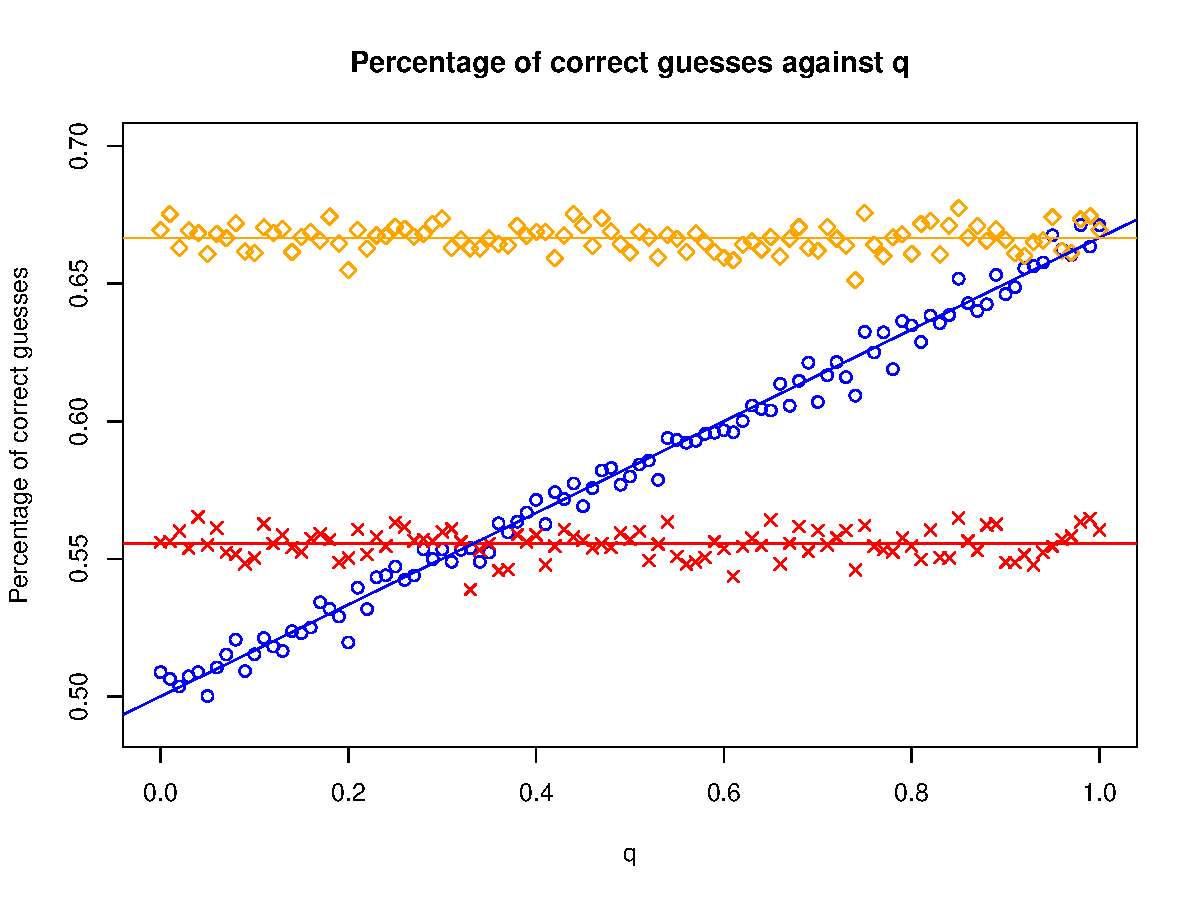
\includegraphics[width=\linewidth]{Figures/MontyHall.pdf}
\caption{Simulation of the probability that strategies $\Psafe_{\1}$ in red, $\Psafe_U$ in blue and $U^*$ in orange result in winning the car. On the horizontal axis the strategy of Monty~Hall $\P[V=2|U=1]=q$ is taken for all $q\in[0,1]$ and on the vertical axis the empirical probability of winning the car is plotted. For each $q$ the amount of Monty~Hall-games simulated are $10000$. The red line and crosses are simulations $\P\left[\Uonesafe=\1_{\{U=1\}}\right]$, the blue line and dots are simulations of $\P[\Usafe=U]$ and the orange line and diamonds are simulations of $\P[U^*=U]$.}
\label{fig:MontyHall}
\end{figure}

All strategies are simulated in figure~\ref{fig:MontyHall} and the code can be found in appendix~\ref{app:MontyHallSim}. The simulation shows that propositions~\ref{prop:MontyHallOpt} and \ref{prop:MontyHallValues} holds in practice. Figure~\ref{fig:MontyHall} also shows that when $q>\frac{1}{3}$, strategy $\Psafe_U$ yields to higher chances of winning the car than $\Psafe_{\1}$. However, strategy $U^*$ outperforms both. Therefore the player should always switch.


We did assume that the car is distributed evenly between the doors at the start and maybe more satisfactory results can be created when dropping this assumption. However, it is more likely that when working with the full model, the No Free Lunch-theorem kicks in and we cannot construct a safe probability as the correct probability is in our model as well. Working without safe probability yields to too many parameters and variables to control, also not resulting into a satisfactory strategy. When one plays the Monty~Hall game, I would advise to always switch your door, how counter-intuitive it may seem.


\section{Two-envelope problem}
The next problem we will cover is the two-envelope problem. We will use the following version of the two-envelope problem. There are two players. The first player, the game master, picks a value $x$ from a non-negative continuous random variable $X$. He then fills one envelope with value $x$ and the other with value $2x$. The second player receives an envelope with uniform probability and observes the value $a$ in that envelope. He is then asked if he wants to keep $a$ or if he wants to switch, possibly gaining $2a$ or gaining a merely $\frac{1}{2}a$.

Let $\X=(0,\infty)$ and $\Y=(0,\infty)^2$. Equip $\X$ with $\Sigma_{\X}=\B((0,\infty))$, the Borel $\sigma$-algebra on $(0,\infty)$. The set $\Y$ is equipped with $\sigma$-algebra
\[\Sigma_{\Y}=\sigma\left(\B\left(\left\{(x,2x)\in\Y\middle|x\in\X\right\}\right)\cup\B\left(\left\{(2x,x)\in\Y\middle|x\in\X\right\}\right)\right),\]
the smallest $\sigma$-algebra containing the Borel $\sigma$-algebras of the lines $y=2x$ and $y=\frac{1}{2}x$. Let $\Omega=\X\times\Y$ be our sample space equipped with $\Sigma=\Sigma_{\X}\times\Sigma_{\Y}$. Let $X$ be a continuous random variable on $\X$ denoting the lowest value of the envelopes and $Y$ be a random variable on $\Y$ denoting the actual values. All probability distributions $\P$ on $(\Omega,\Sigma)$ must be a member of
\[\Pmod=\left\{\P\middle|\P[Y=(x,2x)|X=x]=\P[Y=(2x,x)|X=x]=\frac{1}{2},\E_{\P}[X]<\infty\right\}.\]
Let $A=\pi_1(Y)$ be the value observed by the player and $B=\pi_2(Y)$ be the value in the other envelope, then we would like to know the distribution of $B|A$.

\subsection{Safe probability}
Take again a look at safe probabilities. Using this we can find a safe distribution for $\langle B\rangle|\langle A\rangle$.
\begin{proposition}\label{prop:twoenvelopesafe}
Let $\Pmod$ be our model of probability distributions on $\Omega$. The distribution $\Psafe$ with $\Psafe[B=2a|A=a]=1$ is safe for $\langle B\rangle|\langle A\rangle$ and is the only distribution on $\Omega$ with this property.
\end{proposition}
\begin{proof}
This proof is done by construction. Let $\P\in\Pmod$ be arbitrary. We will first calculate $\E_{\P}[B]:$
\[\E_{\P}[B]=\E_{\P}[\E_{\P}[B|X]]=\int_0^\infty \E_{\P}[B|X=x]f_X(x)dx.\]
Now note that
\[\E_{\P}[B|X=x]=x\P[B=x|X=x]+2x\P[B=2x|X=x]=\frac{x}{2}+x=\frac{3}{2}x.\]
Therefore \[\E_{\P}[B]=\int_0^\infty \E_{\P}[B|X=x]f_X(x)dx=\int_0^\infty\frac{3}{2}xf_X(x)dx=\frac{3}{2}\E_{\P}[X].\]

Now let $\Psafe$ be an arbitrary distribution on $\Omega$. We want to have \[\E_{\P}[\E_{\Psafe}[B|A]]=\E_{\P}[B]=\frac{3}{2}\E_{\P}[X]\] in order for $\Psafe$ to be safe for $\langle B\rangle|\langle A\rangle$. Writing out gives us
\[\E_{\P}[\E_{\Psafe}[B|A]]=\int_0^\infty\E_{\Psafe}[B|A=a]f_A(a)da.\]
We want to write $f_A$ in terms of $f_X$. Considering $\P[A\leq a]$, the only possibilities of $A\leq a$ is when $X\leq a$ and $Y=(a,2a)$ is given or $X\leq \frac{a}{2}$ and $Y=\left(a,\frac{a}{2}\right)$. Writing out yields
\begin{align*}
\P[A\leq a]&=\P[X\leq a,Y=(a,2a)]+\P\left[X\leq\frac{a}{2},Y=\left(a,\frac{a}{2}\right)\right]\\
&=\frac{1}{2}\P[X\leq a]+\frac{1}{2}\P\left[X\leq\frac{1}{2}a\right].
\end{align*}
Differentiating yields \[f_A(a)=\frac{1}{2}f_X(a)+\frac{1}{4}f_X\left(\frac{a}{2}\right).\]
Now take a look at $\E_{\Psafe}[B|A=a]$. Further conditioning on the value of $X$ gives
\begin{align*}
\E_{\Psafe}[B|A=a]&=\E_{\Psafe}[B|X=a,A=a]\Psafe[X=a|A=a]\\
&\phantom{=}+\E_{\Psafe}\left[B\middle|X=\frac{a}{2},A=a\right]\Psafe\left[X=\frac{a}{2}\middle|A=a\right].
\end{align*}
No matter what we choose for $\Psafe$, when $X=a$ and $A=a$ holds, we need to have $B=2a$. Likewise when $A=a$ and $X=\frac{a}{2}$ holds we need $B=\frac{a}{2}$. Therefore we can simplify this expectation value to
\[\E_{\Psafe}[B|A=a]=2a\Psafe[X=a|A=a]+\frac{a}{2}\Psafe\left[X=\frac{a}{2}\middle|A=a\right].\]
Before we can make our final arguments we need to do one change of variables in the integral, as we want to write the whole integral as something multiplied with $f_X(a)$:
\begin{align*}
\E_{\P}[\E_{\Psafe}[B|A]]&=\int_0^\infty\E_{\Psafe}[B|A=a]f_A(a)da\\
&=\int_0^\infty\E_{\Psafe}[B|A=a]\left(\frac{1}{2}f_X(a)+\frac{1}{4}f_X\left(\frac{a}{2}\right)\right)da\\
&=\int_0^\infty\frac{1}{2}\E_{\Psafe}[B|A=a]f_X(a)+\frac{1}{8}\E_{\Psafe}[B|A=2a]f_X\left(a\right)da\\
&=\int_0^\infty f_X(a)\left(\frac{1}{2}\E_{\Psafe}[B|A=a]+\frac{1}{8}\E_{\Psafe}[B|A=2a]\right)da.
\end{align*}
Note that without loss of generality we have
\[\E_{\Psafe}[B|A=2a]=4a\Psafe[X=2a|A=2a]+a\Psafe\left[X=a\middle|A=2a\right].\]
When the player observes a value from $A$, he does not know whether he is in the situation $A=a$ or $A=2a$. Therefore we'd like to treat both cases equally and impose
\[\Psafe[X=a|A=a]=\Psafe[X=2a|A=2a]=p\]
with $p\in[0,1]$. This results to
\begin{align*}
\frac{1}{2}\E_{\Psafe}[B|A=a]+\frac{1}{8}\E_{\Psafe}[B|A=2a]&=ap+\frac{a}{4}(1-p)+\frac{a}{2}p+\frac{a}{8}(1-p).
\end{align*}
Since we need $\E_{\P}[\E_{\Psafe}[B|A]]=\E_{\P}[B]=\frac{3}{2}\E_{\P}[X]$, the only $p$ for which this equality is satisfied is $p=1$. This results to
\[\E_{\P}[\E_{\Psafe}[B|A]]=\int_0^\infty f_X(a)\left(a+\frac{a}{2}\right)da=\frac{3}{2}\E_{\P}[X]=\E_{\P}[B],\]
which is what we needed.
\end{proof}

Note that the $\Psafe$ from proposition~\ref{prop:twoenvelopesafe} is not safe for $\langle B\rangle|[A]$, as we need $\frac{3}{2}\E_{\P}[X]=\E_{\Psafe}[B|A=a]=2a$ for all $\P\in\Pmod$ and $a\in(0,\infty)$ in this case. This is clearly not possible as the only restriction on $\E_{\P}[X]$ imposed by $\Pmod$ is that $\E_{\P}[X]$ is finite.

Consider now the random variable $\EnvIndSafe$. This random variable describes whether the second envelope has twice the observed value. If a safe distribution of $\EnvIndSafe|A$ exist, we can use it to devise a strategy in the two envelope game.

In our setting it is wise to find out whether $\EnvIndSafe$ is a pivot for $B|A$. However, take $a\in (0,\infty)$ arbitrary, then 
\[\range(B|A=a)=\left\{\frac{a}{2},2a\right\}\]
is a set with two elements and no interval. Thus definition~\ref{def:contpivot} cannot be applied here and no pivot of $B|A$ exists.

However, this does not stop us from searching for a safe distribution $\Psafe$ for $\EnvIndSafe|A$ or one of the variants in definitions~\ref{def:safeprop} and \ref{def:strongsafeprop}.
\begin{proposition}\label{prop:TwoEnvelopeIndSafe}
A distribution $\Psafe$ on $\Omega$ is safe for $\langle\EnvIndSafe\rangle|\langle A\rangle$ in model $\Pmod$ if
\[\int_0^\infty \Psafe[B=2A|A=a]f_A(a)da=\frac{1}{2}\]
holds where $f_A$ is the density function of $A$.

The distribution $\Psafe$ with $\Psafe[B=2A|A=a]=\frac{1}{2}$ is the only safe distribution for $\langle\EnvIndSafe\rangle|[A]$ and $\EnvIndSafe|[A]$.
\end{proposition}
\begin{proof}
This proof is by construction. Let $\Psafe\in\Pmod$ be arbitrary. We will start with $\langle\EnvIndSafe\rangle|\langle A\rangle$. Firstly we have
\begin{align*}
\E_{\P}\left[\EnvIndSafe\right]&=\P[B=2A]=\int_0^\infty\P[B=2X|X=x]f_X(x)dx\\
&=\frac{1}{2}\int_0^\infty f_X(x)dx=\frac{1}{2},
\end{align*}
as $B=2A$ only happens when $A=X$ and $\P[B=2X|X=x]=\frac{1}{2}$ is dictated by our model $\Pmod$. Let $a\in(0,\infty)$ be arbitrary, then
\[\E_{\Psafe}\left[\EnvIndSafe\middle|A=a\right]=\Psafe[B=2A|A=a]\]
must hold. Therefore we have
\[\E_{\P}\left[\E_{\Psafe}\left[\EnvIndSafe\middle|A=a\right]\right]=\int_0^\infty\Psafe[B=2A|A=a]f_A(a)da.\]
The density $f_A$ of $A$ is unknown. We do know that $\Psafe$ must be safe for $\langle\EnvIndSafe\rangle|\langle A\rangle$ by definition~\ref{def:safeprop}, thus we need $\E_{\P}\left[\E_{\Psafe}\left[\EnvIndSafe\middle|A=a\right]\right]=\E_{\P}\left[\EnvIndSafe\right]$. This results to the requirement
\[\int_0^\infty\Psafe[B=2A|A=a]f_A(a)da=\frac{1}{2}.\]

Now we'll move our focus to safety for $\langle\EnvIndSafe\rangle|[A]$. Since for all $a\in(0,\infty)$ we have $\E_{\Psafe}\left[\EnvIndSafe\middle|A=a\right]=\Psafe[B=2A|A=a]$, we immediately see that $\Psafe[B=2A|A=a]=\frac{1}{2}$ must hold for $\Psafe$ in order to be safe for $\langle\EnvIndSafe\rangle|[A]$.

Proposition~\ref{prop:safeproperties} states that a distribution $\Psafe$ is safe for $\EnvIndSafe|[A]$ if and only if $\P[B=2A]=\Psafe[B=2A|A=a]$ holds for all $\P\in\Pmod$ and $a\in(0,\infty)$. This requirement only satisfied when $\Psafe[B=2A|A=a]=\frac{1}{2}$ holds for all $a\in(0,\infty)$ as $\P[B=2A]=\frac{1}{2}$ holds by our model $\Pmod$. Proposition~\ref{prop:safeimply} lastly gives us that this is the only possible $\Psafe$ that is safe for $\EnvIndSafe|[A]$.
\end{proof}

Therefore safe probability considered we can estimate the distribution of $\EnvIndSafe|A$ best by $\Psafe[B=2A|A=a]=\frac{1}{2}$ from proposition~\ref{prop:TwoEnvelopeIndSafe}.

As we now have two different safe probabilities that can be used to give an advice on whether the player must switch, we can take a look at which distribution predicts better. The result, however, is that when predicts $\EnvIndSafe|A$ using $\Psafe[B=2A|A=a]=q$, then for all $q\in[0,1]$ the player wins on average the same amount of money and predicts the value of $\EnvIndSafe$ correctly with probability $\frac{1}{2}$. This is explored further in the following proposition.

\begin{proposition}\label{prop:TwoEnvelopePropHalf}
Let $q\in[0,1]$ and suppose we predict the value of $\EnvIndSafe|A$ by $\Psafe[B=2A|A=a]=q$ for all $a\in(0,\infty)$. Let $\EnvIndSafe^*$ denote that prediction. Then for all $\P\in\Pmod$ we have
\begin{align*}
\P\left[\EnvIndSafe^*=\EnvIndSafe\right]&=\frac{1}{2},&\E_{\P}[W]=\frac{3}{2}\E_{\P}[X].
\end{align*}
Let $\tilde{W}$ be the value won after a round by predicting using $\EnvIndSafe^*$, then for all $\P\in\Pmod$ we have $\E_{\P}[\tilde{W}]=\frac{3}{2}\E_{\P}[X]$.
\end{proposition}
\begin{proof}
Let $\P\in\Pmod$ be arbitrary. Consider $\EnvIndSafe^*$ first. The random variables $\EnvIndSafe^*$ and $\EnvIndSafe$ are independent as the value of $\EnvIndSafe$ is not known when predicting $\EnvIndSafe^*$. Writing out gives
\begin{align*}
&\phantom{=}\P\left[\EnvIndSafe^*=\EnvIndSafe\right]\\
&=\sum_{x\in\{0,1\}}\P\left[\EnvIndSafe^*=\EnvIndSafe\middle|\EnvIndSafe=x\right]\P\left[\EnvIndSafe=x\right]\\
&=\frac{1}{2}(1-q)+\frac{1}{2}\cdot q=\frac{1}{2},
\end{align*}
as $\P[B=2A]=\P[B\neq2A]=\frac{1}{2}$ by $\P\in\Pmod$ and 
\[\P\left[\EnvIndSafe^*=\EnvIndSafe\middle|\EnvIndSafe=1\right]=\P\left[\EnvIndSafe^*=1\right]=q.\]

If $\tilde{W}$ is predicted by $\EnvIndSafe^*$, then $\tilde{W}=qB+(1-q)A$ must hold as $\EnvIndSafe^*$ is predicted by $\Psafe[B=2A|A=a]=q$. This results into
\[\E_{\P}[\tilde{W}]=q\E_{\P}[B]+(1-q)\E_{\P}[A].\]
The proof of proposition~\ref{prop:twoenvelopesafe} already calculated $\E_{\P}[B]=\frac{3}{2}\E_{\P}[X]$ and without loss of generality $\E_{\P}[A]=\frac{3}{2}\E_{\P}[X]$ holds as well. Therefore
\[\E_{\P}[\tilde{W}]=q\E_{\P}[B]+(1-q)\E_{\P}[A]=\frac{3q}{2}\E_{\P}[X]+\frac{3(1-q)}{2}\E_{\P}[X]=\frac{3}{2}\E_{\P}[X].\]
\end{proof}

This proposition can be immediately applied to our safe probability distributions.

\begin{corollary}
Let $\tilde{B}$ be the prediction of $B|A$ according to the $\Psafe$ that is safe for $B|[A]$ from proposition~\ref{prop:twoenvelopesafe} and $\tilde{\1}_{\{B=2A\}}$ be the prediction of $\EnvIndSafe|A$ according to the $\Psafe$ that is safe for $\EnvIndSafe|[A]$ from proposition~\ref{prop:TwoEnvelopeIndSafe}. Let $\P\in\Pmod$ be arbitrary, then
\[\P\left[\tilde{\1}_{\{B=2A\}}=\EnvIndSafe\right]=\P[\tilde{B}=B]=\frac{1}{2}.\]
\end{corollary}
\begin{proof}
Consider $\tilde{\1}_{\{B=2A\}}$ first. Directly applying proposition~\ref{prop:TwoEnvelopePropHalf} with $q=\frac{1}{2}$ results to $\P\left[\tilde{\1}_{\{B=2A\}}=\EnvIndSafe\right]=\frac{1}{2}$.

Now we will move on to $\P[\tilde{B}=B]$. There are two possible proofs. The value of $\tilde{B}$ is predicted by $\Psafe[B=2a|A=a]=1$ and since $B$ can only take two different values when $A$ is known, proposition~\ref{prop:TwoEnvelopePropHalf} can be applied with $q=1$ to get $\P[\tilde{B}=B]=\frac{1}{2}$.\\
A different proof involves conditioning on the value of $A$ and the value of $B$, which yields
\begin{align*}
\P[\tilde{B}=B]&=\int_0^\infty\P[\tilde{B}=B|A=a]f_A(a)da\\
&=\int_0^\infty\sum_{b\in\left\{\frac{a}{2},2a\right\}}\P[\tilde{B}=B|B=b,A=a]\P[B=b|A=a]f_A(a)da.
\end{align*}
Our model $\Pmod$ dictates $\P[B=b|A=a]$ for all $a\in(0,\infty)$ and $b\in\left\{\frac{a}{2},2a\right\}$. Furthermore, we always predict that $\tilde{B}$ is twice the value of $A$, thus
\begin{align*}
\P[\tilde{B}=B|B=2a,A=a]&=\P[\tilde{B}=2a|A=a]=1,\\
\P\left[\tilde{B}=B\middle|B=\frac{a}{2},A=a\right]&=\P\left[\tilde{B}=\frac{a}{2}|A=a\right]=0.
\end{align*}
This results to \[\P[\tilde{B}=B]=\int_0^\infty f_A(a)\left(1\cdot\frac{1}{2}+0\cdot\frac{1}{2}\right)da=\frac{1}{2}.\]
\end{proof}

Proposition~\ref{prop:TwoEnvelopePropHalf} tells us that when $\EnvIndSafe$ is predicted by a prediction $\Psafe$ which ignores the value of $A$, every such prediction yields equal results no matter the choice of $\Psafe$. The player on average wins $\frac{3}{2}\E_{\P}[X]$, where here $\P$ is the actual distribution of $X$. Strategies able to improve upon $\Psafe$ and obtaining higher average $\frac{3}{2}\E_{\P}[X]$ have to take the value of $A$ into account. Such strategies are strategies that have a decreasing probability of switching to envelope $B$ the higher the value of $A$ is observed, as \cite{McDonnell09,Abbott10,McDonnell11,Egozcue15} have pointed out. Such strategy $\Psafe$ can only be safe for $\langle\1_{\{B=2A\}}\rangle|\langle A\rangle$ and has to fulfil the requirement
\[\int_0^\infty \Psafe[B=2A|A=a]f_A(a)da=\frac{1}{2}\] by proposition~\ref{prop:TwoEnvelopeIndSafe}, where $f_A$ is the actual density of $A$. This density is most of the times not known to the player, making it impossible to guess a safe probability distribution when playing the two envelope game in real life.

Furthermore, if a strategy with decreasing probability in observed $A$ is chosen, then there is no guarantee how much better it performs than $\frac{3}{2}\E_{\P}[X]$. The only requirement on the distribution of $X$ is that it has finite expectation value, thus when the game master puts that expectation value in an interval where the player's strategy already dictates almost $0$ probability of switching, the player is still left with $\frac{3}{2}\E_{\P}[X]$.

We observe that with the two envelope problem, safe probability dictates a strategy that wins a consistent value. That strategy can be improved, however it is not possible to know how much such improvement actually results in winning more.

\section{Dice game}
Another problem that uses the same techniques is the dice game. In het dice game, a fair die is cast. The game master observes its value and tells the player whether the dies value is in the set $\{1,2,3,4\}$ or in the set $\{3,4,5,6\}$. The player must then guess the probability of the die having the value $3$.

This dice game serves two purposes. It can be used to explain safe probabilities instead of the Monty Hall game, as the dice game is purely mathematical and removes the distractions the Monty Hall game has. This is the reason why \cite{Grunwald13} originally conceived this game. The second reason is that the game master can play two different strategies, namely the frequency of saying $\{3,4,5,6\}$ when observing either $3$ or $4$. The safe probability distribution now is not a single distribution, but becomes a member of a solution set of linear equations.

We will adopt the notation of \cite{Grunwald13} for working out this problem. Let $\Y=\{1,2,3,4,5,6\}$ be our outcome space and let $\X=\{\{1,2,3,4\},\{3,4,5,6\}\}$ be our space of observations. The probability space is then $\mathcal{Z}=\X\times\Y$. Let $Y$ be a random variable on $\Y$ denoting the value of the die and let $X$ be a random variable on $\X$ denoting which set the game master told us. For our model $\Pmod$ we assume the die is fair, thus $\P[Y=y]=\frac{1}{6}$ for all $y\in\Y$ and we assume the game master does not lie, thus $\P[Y\in x|X=x]=1$ must hold for all $x\in\X$. Therefore, we use the following model:
\[\Pmod=\left\{\P\middle|\forall y\in\Y:\P[Y=y]=\frac{1}{6},\forall x\in\X:\P[Y\in x|X=x]=1\right\}.\]
For shorthand purposes we will write $x_2=\{1,2,3,4\}$ and $x_2=\{3,4,5,6\}$ such that $\X=\{x_1,x_2\}$.

\begin{example}[Dilated probabilities \cite{Grunwald13}]
Let $p,q\in[0,1]$ and suppose the game master chose $\P\in\P^*$ such that $\P[X=\{3,4,5,6\}|Y=3]=p$ and $\P[X=\{3,4,5,6\}|Y=4]=q$. Then \cite{Grunwald13} calculated that 
\[\P[Y=6|X=\{3,4,5,6\}]=\frac{1}{p+q+2},\]
showing that the probability of rolling $6$ when told that the die has value in $\{3,4,5,6\}$ dilates from $\frac{1}{4}$ to $\frac{1}{2}$, depending on the game masters strategy. The game master was forced to tell the player $\{3,4,5,6\}$ as he cannot lie, however from the strategies imposed when rolling $3$ or $4$ the player is still not sure how likely a roll of $6$ is.
\end{example}

We will now approach the dice game using safe probabilities.

\begin{proposition}
Let $\X$, $\Y$, $\mathcal{Z}$, $X$, $Y$ and $\Pmod$ be as before. A distribution $\Psafe$ on $\mathcal{Z}$ is safe for $\langle Y\rangle|\langle X\rangle$ and $\langle Y\rangle|[X]$ if it is a member of the set 
\[\tilde{\mathcal{P}}=\left\{\Psafe\middle|
\begin{array}{l}
\Psafe[Y=1|X=x_1]=\Psafe[Y=2|X=x_1],\\
\Psafe[Y=3|X=x_1]=\frac{1}{2}-5\Psafe[Y=1|X=x_1],\\
\Psafe[Y=5|X=x_2]=\Psafe[Y=6|X=x_2],\\
\Psafe[Y=3|X=x_2]=3\Psafe[Y=5|X=x_2]+\frac{1}{2},\\
\Psafe[Y=1|X=x_1],\Psafe[Y=5|X=x_1]\in\left[0,\frac{1}{10}\right]
\end{array}
\right\}.\]
There exists no safe distribution for $Y|[X]$.
\end{proposition}
\begin{proof}
The proof is by construction. Let $\Psafe$ be an arbitrary distribution. Let $\P\in\Pmod$ be such that there are $p,q\in[0,1]$ with $\P[X=x_2|Y=3]=p$ and $\P[X=x_2|Y=4]=q$.

We first focus on safety for $\langle Y\rangle|\langle X\rangle$, thus $\E_{\P}[\E_{\Psafe}[Y|X]]=\E_{\P}[Y]$. The right-hand side is easy to compute:
\[\E_{\P}[Y]=\sum_{y=1}^6 y\P[Y=y]=\frac{1+2+3+4+5+6}{6}=\frac{7}{2}.\]
For $\E_{\P}[\E_{\Psafe}[Y|X]]$, we first focus on $\P[X=x_2]$. Conditioning on $Y$ yields
\[\P[X=x_2]=\sum_{y=1}^6\P[X=x_2|Y=y]\P[Y=y]=\frac{1}{6}\sum_{y=1}^6\P[X=x_2|Y=y].\]
The game master cannot lie, thus $\P[X=x_2|Y=5]=\P[X=x_2|Y=6]=1$ and $\P[X=x_2|Y=1]=\P[X=x_2|Y=2]=0$ immediately hold. We further have $\P[X=x_2|Y=3]=p$ and $\P[X=x_2|Y=4]=q$, thus the value of $\P[X=x_2]$ is
\[\P[X=x_2]=\frac{1}{6}\sum_{y=1}^6\P[X=x_2|Y=y]=\frac{2}{3}+\frac{p+q}{6}.\]
Since $\X$ only has two elements, $\P[X=x_1]=\frac{1}{3}-\frac{p+q}{6}$ follows. We can now write out $\E_{\P}[\E_{\Psafe}[Y|X]]$, however we must shorten our notation. Let $\Psafe[y|x]$ denote $\Psafe[Y=y|X=x]$ for all $(x,y)\in\mathcal{Z}$. Writing out yields
\begin{align*}
\E_{\P}[\E_{\Psafe}[Y|X]]&=\E_{\Psafe}[Y|X=x_1]\P[X=x_1]+\E_{\Psafe}[Y|X=x_2]\P[X=x_2]\\
&=\left(\Psafe(1|x_1)+2\Psafe(2|x_1)+3\Psafe(3|x_1)+4\Psafe(4|x_1\right)\left(\frac{2}{3}-\frac{p+q}{6}\right)\\
&\phantom{=}+\left(3\Psafe(3|x_2)+4\Psafe(4|x_2)+5\Psafe(5|x_2)+6\Psafe(6|x_2\right)\left(\frac{1}{3}+\frac{p+q}{6}\right)\\
&=\frac{p+q}{6}\left(\sum_{y=3}^{6}y\Psafe[y|x_2]-\sum_{y=1}^4y\Psafe[y|x_1]\right)+\sum_{y=1}^4\frac{2y}{3}\Psafe[y|x_1]\\
&\phantom{=}+\sum_{y=3}^6\frac{y}{3}\Psafe[y|x_2].
\end{align*}
As we have $\E_{\P}[Y]=\frac{1}{6}$, we need to get rid of the dependence on $p+q$. This results into the condition
\[\sum_{y=3}^{6}y\Psafe[y|x_2]=\sum_{y=1}^4y\Psafe[y|x_1].\]
When this condition is satisfied, we need \[\sum_{y=1}^4\frac{2y}{3}\Psafe[y|x_1]+\sum_{y=3}^6\frac{y}{3}\Psafe[y|x_2]=\frac{7}{2}\] for $\Psafe$ to be safe for $\langle Y\rangle|\langle X\rangle$. We impose one further assumption on our safe probability to reduce the amount of possible safe probabilities. Suppose the die shows $5$ or $6$, the game master has to tell $x_2$. Thus it is logical to assume that $\Psafe[5|x_2]=\Psafe[6|x_2]$ and $\Psafe[1|x_1]=\Psafe[2|x_1]$, as when an $x_2$ is revealed there is no reason why $5$ is preferred more than $6$. Also as the game master cannot lie, \[\Psafe[5|x_1]=\Psafe[6|x_1]=\Psafe[1|x_2]=\Psafe[2|x_2]=0\] can be assumed. This all results into the following system of equations:
\[\begin{pmatrix}
\frac{2}{3}&\frac{4}{3}&2&\frac{8}{3}&1&\frac{4}{3}&\frac{5}{3}&2\\
-1&-2&-3&-4&3&4&5&6\\
1&-1&0&0&0&0&0&0\\
0&0&0&0&0&0&1&-1\\
1&1&1&1&0&0&0&0\\
0&0&0&0&1&1&1&1
\end{pmatrix}\begin{pmatrix}
\Psafe[1|x_1]\\\Psafe[2|x_1]\\\Psafe[3|x_1]\\\Psafe[4|x_1]\\
\Psafe[3|x_2]\\\Psafe[4|x_2]\\\Psafe[5|x_2]\\\Psafe[6|x_2]
\end{pmatrix}=\begin{pmatrix}
\frac{7}{2}\\0\\0\\0\\1\\1
\end{pmatrix}.
\]
The set $\tilde{\mathcal{P}}$ is the set of all solutions to this system. As $\Psafe$ needs to be a valid probability distribution, we need to have $\Psafe[y|x]\in[0,1]$ for all $(x,y)\in\mathcal{Z}$. We have
\begin{align*}
\Psafe[3|x_1]&=3\Psafe[1|x_1]+\frac{1}{2},\\
\Psafe[4|x_1]&=5\Psafe[1|x_1]-\frac{1}{2},
\end{align*}
thus $\Psafe[3|x_1]\in[0,1]$ holds when $\Psafe[1|x_1]\in\left[0,\frac{1}{6}\right]$ and $\Psafe[4|x_1]\in[0,1]$ holds when $\Psafe[1|x_1]\in\left[0,\frac{1}{10}\right]$. Without loss of generality $\Psafe[5|x_2]\in\left[0,\frac{1}{10}\right]$ must hold as well. This proves the last requirement $\Psafe[1|x_2],\Psafe[5|x_2]\in\left[0,\frac{1}{10}\right]$ from $\tilde{\mathcal{P}}$ and completes our proof that $\tilde{\mathcal{P}}$ contains all probability distributions that are safe for $\langle Y\rangle|\langle X\rangle$.

We will now focus on safety for $\langle Y\rangle|[X]$. Note that a safe distribution must be an element of $\tilde{\mathcal{P}}$ by proposition~\ref{prop:safeimply}. All distributions $\Psafe\in\tilde{\mathcal{P}}$ have the requirement
\[\E_{\Psafe}[Y|X=x_2]=\sum_{y=3}^{6}y\Psafe[y|x_2]=\sum_{y=1}^4y\Psafe[y|x_1]=\E_{\Psafe}[Y|X=x_1],\]
thus we only need to prove that $\E_{\Psafe}[Y|X=x_2]=\frac{7}{2}$ holds. Writing out and using properties of $\Psafe$ results to
\begin{align*}
\E_{\Psafe}[Y|X=x_2]&=3\left(3\Psafe[5|x_2]+\frac{1}{2}\right)+4\left(\frac{1}{2}-5\Psafe[5|x_2]\right)+11\Psafe[5|x_2]\\
&=\frac{7}{2}+20\Psafe[5|x_2]-20\Psafe[5|x_2]=\frac{7}{2},
\end{align*}
proving that all distributions in $\tilde{\mathcal{P}}$ are safe for $\langle Y\rangle|[X]$ as well.

Lastly we turn to safety for $Y|[X]$. This requires $\Psafe[1|x_1]=\P[Y=1]$ for all $\P\in\Pmod$. A safe distribution must come from $\tilde{\mathcal{P}}$ according to definition~\ref{def:strongsafeprop}, thus pick $\Psafe\in\tilde{\mathcal{P}}$ arbitrarily. Proposition~\ref{prop:safeproperties} implies $\Psafe[1|x_1]=\frac{1}{6}$, which is a clear contradiction to $\Psafe[1|x_1]\in\left[0,\frac{1}{10}\right]$. Thus there is no distribution $\Psafe$ on $\mathcal{Z}$ that is safe for $Y|[X]$.
\end{proof}

Thus instead of the safe distribution having a single and defining condition like the Monty Hall game or the two envelope problem, the safe distribution is a member of a set of safe distributions, where all can be played to nullify the game masters strategy and having the same average as the die.

We now have a safe distribution simulating an average die roll, however we were asked to guess what the probability of rolling $3$ is when either $x_1$ or $x_2$ is revealed. This can be best done by considering the random variable $\DieInd$, as safety for $\langle\DieInd\rangle|[X]$ implies
\[\P[Y=3]=\E_{\P}[\DieInd]=\E_{\Psafe}[\DieInd|X=x]=\Psafe[Y=3|X=x]\]
for all $\P\in\Pmod$ and $x\in\X$.
\begin{proposition}\label{prop:DiceIndSafe}
Let $\X$, $\Y$, $\mathcal{Z}$, $X$, $Y$ and $\Pmod$ be as before. A distribution $\Psafe$ on $\mathcal{Z}$ is safe for $\DieInd|[X]$ when $\Psafe[Y=3|X=x_1]=\Psafe[Y=3|X=x_2]=\frac{1}{6}$ holds. A distribution $\Psafe$ can only be safe for $\langle\DieInd\rangle|\langle X\rangle$ and $\langle\DieInd\rangle|[X]$ if it has this requirement as well.

The same holds for $\1_{\{Y=4\}}$ instead of $\1_{\{Y=3\}}$.
\end{proposition}
\begin{proof}
The proof is by construction. Let $\Psafe$ be an arbitrary distribution. Let $\P\in\Pmod$ be such that there are $p,q\in[0,1]$ with $\P[X=x_2|Y=3]=p$ and $\P[X=x_2|Y=4]=q$. We already calculated that
\begin{align*}
\P[X=x_1]&=\frac{2}{3}-\frac{p+q}{6},&\P[X=x_2]&=\frac{1}{3}+\frac{p+q}{6}.
\end{align*}
Use the shorthand $\Psafe[y|x]=\Psafe[Y=y|X=x]$ for all $(x,y)\in\mathcal{Z}$. Writing out $\E_{\P}[\E_{\Psafe}[\DieInd|X]]$ results to
\begin{align*}
\E_{\P}[\E_{\Psafe}[\DieInd|X]]&=\sum_{x\in\{x_1,x_2\}}\E_{\Psafe}[\DieInd|X=x]\P[X=x]\\
&=\Psafe[3|x_1]\left(\frac{2}{3}-\frac{p+q}{6}\right)+\Psafe[3|x_2]\left(\frac{1}{3}+\frac{p+q}{6}\right)\\
&=\frac{p+q}{6}\left(\Psafe[3|x_2]-\Psafe[3|x_1]\right)+\frac{2}{3}\Psafe[3|x_1]+\frac{1}{3}\Psafe[3|x_2].
\end{align*}
As $\E_{\P}[\E_{\Psafe}[\DieInd|X]]=\frac{1}{6}$ must hold, we need the condition $\Psafe[3|x_2]=\Psafe[3|x_1]$ for $\E_{\P}[\E_{\Psafe}[\DieInd|X]]$ to remain constant when $p$ and $q$ changes. Filling in this condition results to $\E_{\P}[\E_{\Psafe}[\DieInd|X]]=\Psafe[3|x_1]=\frac{1}{6}$, proving that the condition $\Psafe[3|x_1]=\Psafe[3|x_2]=\frac{1}{6}$ is necessary for safety $\Psafe$ to be safe for $\langle\DieInd\rangle|\langle X\rangle$.

Testing this $\Psafe$ for safety for $\langle\DieInd\rangle|[X]$ yields
\begin{align*}
\E_{\Psafe}[\DieInd|X=x_1]&=\Psafe[Y=3|X=x_1]=\frac{1}{6}=\P[Y=3],\\
\E_{\Psafe}[\DieInd|X=x_2]&=\Psafe[Y=3|X=x_2]=\frac{1}{6}=\P[Y=3],
\end{align*}
thus $\Psafe$ is safe for $\langle\DieInd\rangle|[X]$ as well.

Lastly we turn our attention to safety for safety for $\DieInd|[X]$. We need $\P[\DieInd=i]=\Psafe[\DieInd=i|X=x]$ for all $i\in\{0,1\}$ and $x\in\X$. Pick a $\Psafe$ that is safe for $\langle\DieInd\rangle|[X]$.
\begin{itemize}
	\item[$i=0$:] Let $i=0$ and $x\in\X$, then we have $\P[\DieInd=1]=\P[Y\neq3]=\frac{5}{6}$. We also have \[\Psafe[\DieInd=0|X=x]=\Psafe[Y\neq 3|X=x]=1-\Psafe[\DieInd=1|X=x]=\frac{5}{6}.\] Thus this requirement is fulfilled.
	\item[$i=1$:] Let $i=1$ and $x\in\X$, then we already have \[\P[\DieInd=1]=\P[Y=3]=\Psafe[Y=3|X=x]=\Psafe[\DieInd=1|X=x].\]
\end{itemize}
Therefore this $\Psafe$ is safe for $\DieInd|[X]$ as well.

Without loss of generality the whole proof holds for $\1_{\{Y=4\}}$ as well.
\end{proof}

Note that $\DieInd$ cannot be a pivot for $Y|X$. This is clear when checking definition~\ref{def:discpivot}. Define $f$ with $f(Y,X)=\DieInd$, then $f_{x_1}(1)=f_{x_1}(2)=0$ making $f_{x_1}$ not injective.

We will lastly check whether we can say something about safety for $\1_{\{Y=y\}}|X$ with $y\in\{1,2,5,6\}$. Unfortunately, there are no safe distributions in this case.
\begin{proposition}
There is no safe probability distribution for $\langle\1_{\{Y=y\}}\rangle|\langle X\rangle$ with $y\in\{1,2,5,6\}$.
\end{proposition}
\begin{proof}
Pick $y=1$. As $X=x_1$ is the only possible option when rolling $1$, we have
\begin{align*}
\E_{\P}[\E_{\Psafe}[\1_{\{Y=1\}}|X]]&=\Psafe[Y=1|X=x_1]\P[X=x_1]\\
&=\Psafe[Y=1|X=x_1]\left(\frac{2}{3}-\frac{p+q}{6}\right).
\end{align*}
We need $\E_{\P}[\E_{\Psafe}[\1_{\{Y=1\}}|X]]=\P[Y=1]=\frac{1}{6}$, but there is no possible value for $\Psafe[Y=1|X=x_1]$ such that 
\[\Psafe[Y=1|X=x_1]\left(\frac{2}{3}-\frac{p+q}{6}\right)=\frac{1}{6}\]
holds for all $p,q\in[0,1]$.

This proof applies to all $y\in\{1,2,5,6\}$, where in the case of $y\in\{5,6\}$ we need to condition on $X=x_2$ instead of $X=x_1$. 
\end{proof}

\section{Boy or girl problem}
Another paradox that can be studied using safe probabilities is the boy or girl problem. A stranger approaches you and you two get in conversation. The stranger tells you that he has two children and at least one of them is a girl. You want to know what the probability is that the has two girls.

The paradox arises when one misinterpreted the setting. Suppose you ask the stranger if he has at least one girl. If he says yes, the probability of two girls is $\frac{1}{3}$, as he can also have a boy and a girl and you do not know whether the earlier mentioned girl is his oldest child. This calculation is not controversial, as his answer yes implies the set of possibilities $\{bg, gb, gg\}$ and is answer no implies the set of possibilities $\{bb\}$. These sets do not overlap, thus Bayesian probability theory can be applied without any problems.\\
Suppose now the strangers tells you out of the blue that he has two children and at least one of them is a girl. Now the setting changes, as he could also have told you that at least one of his child is a boy. If he said he has a girl, the set of possibilities is $\{bg, gb, gg\}$ and if he said he has a boy, the set of possibilities is $\{bg, gb, bb\}$. Now there is an overlap of $\{bg, gb\}$ and Bayesian probability theory does not hold any-more. The probability of the stranger having two girls given he said he has at least one is now dilated between $0$ and $\frac{1}{3}$, dependent on the willingness of the stranger to reveal he has a girl.

We will now build our model. Let $\X=\{b,g\}$ be our observation space and $\Y=\{bb,bg, gg\}$ be our space of outcomes. We do not care about whether the girl is older than the boy in the event that the stranger has a boy and a girl, thus we remove the outcome $gb$. Let $U$ be a random variable on $\Y$ denoting the children of the stranger and $V$ be a random variable on $\X$ denoting whether the stranger told you he as at least one boy ($V=b$) or at least one girl ($V=g$). Our probability space is $\mathcal{Z}=\X\times\Y$ and all probabilities $\P$ on $\mathcal{Z}$ must be in
\[\Pmod=\left\{\P|\P[U=bb]=\frac{1}{4},\P[U=bg]=\frac{1}{2},\P[V=g]\in[0,1]\right\}.\]
Since $U$ is not real-valued, we cannot calculate $\E_{\P}[U]$ for any $U\in\Pmod$. Thus there is no notion of safety for $U|V$. We can speak of safety for $\ChildInd|V$, as the event $U=bg$ arises both in conditioning on $V=b$ and $V=g$.
\begin{proposition}\label{prop:childsafe}
Let $\X$, $\Y$, $\mathcal{Z}$, $U$, $V$ and $\Pmod$ be as above. A distribution $\Psafe$ is safe for $\langle\ChildInd\rangle|\langle V\rangle$, $\langle\ChildInd\rangle|[V]$, $\ChildInd|\langle V\rangle$ or $\ChildInd|[V]$ only if \[\Psafe[U=bg|V=v]=\frac{1}{2}\] for all $v\in\X$ holds.
\end{proposition}
\begin{proof}
We will proof safety for $\langle\ChildInd\rangle|\langle V\rangle$ by construction. Then safety for $\ChildInd|[V]$ needs a mere check of the distribution constructed and safety for $\langle\ChildInd\rangle|[V]$ then follows from definition~\ref{def:strongsafeprop}.

Let $\P\in\Pmod$ be arbitrary. Let $\Psafe$ be an arbitrary distribution on $\mathcal{Z}$. Firstly we have
\[\E_{\P}[\ChildInd]=\P[U=bg]=\frac{1}{2}.\]
Let $p\in[0,1]$ be such that $\P[V=g]=p$ holds. Secondly we have
\begin{align*}
\E_{\Psafe}[\ChildInd|V=b]&=\Psafe[U=bg|V=b]\P[V=b]=(1-p)\Psafe[U=bg|V=b],\\
\E_{\Psafe}[\ChildInd|V=g]&=\Psafe[U=bg|V=g]\P[V=g]=p\Psafe[U=bg|V=g].\\
\end{align*}
Therefore we have
\begin{align*}
\E_{\P}[\E_{\Psafe}[\ChildInd|V]]&=p\left(\Psafe[U=bg|V=g]-\Psafe[U=bg|V=b]\right)\\
&\phantom{=}+\Psafe[U=bg|V=b].
\end{align*}
Since $\E_{\P}[\ChildInd]$ is constant, we need $\Psafe[U=bg|V=g]=\Psafe[U=bg|V=b]$. Then we have
\[\frac{1}{2}=\E_{\P}[\ChildInd]=\Psafe[U=bg|V=b],\]
forcing  $\Psafe[U=bg|V=b]=\frac{1}{2}$. Therefore a safe distribution for $\langle\ChildInd\rangle|\langle V\rangle$ must have $\Psafe[U=bg|V=v]=\frac{1}{2}$ for all $v\in\X$.

Take now a look at safety for $\ChildInd|[V]$. We have
\begin{align*}
\P[U=bg]=\frac{1}{2}=\Psafe[U=bg|V=b],\\
\P[U=bg]=\frac{1}{2}=\Psafe[U=bg|V=g],
\end{align*}
thus $\Psafe$ is safe for $\ChildInd|[V]$ as well. Now $\Psafe$ is also safe for $\langle\ChildInd\rangle|[V]$ and $\ChildInd|\langle V\rangle$ by definition~\ref{def:strongsafeprop} and proposition~\ref{prop:safeimply}.
\end{proof}
\subsection{Boy or girl problem 2.0}
There is a second variant of the boy or girl problem stated in a lecture by Peter Grünwald. He stated a revised boy or girl problem as such:
\begin{enumerate}
	\item A person is picked uniformly at random from a population and a conversation is started.
	\item You ask if at least one of his children is a boy. Suppose his answer is yes, then the probability of two boys if $\frac{1}{3}$. As stated in the previous section, this is not controversial.
	\item You ask if he can give you the name of his son. He can choose which son if he has two. The answer is `Martin'.
	\item You ask if Martin is his youngest child.
	\begin{itemize}
		\item[yes:] If he answered yes, then his youngest child is a boy and the probability of two boys is now $\frac{1}{2}$.
		\item[no:] If he answered no, then his oldest child is a boy and the probability of two boys is now $\frac{1}{2}$.
	\end{itemize}
\end{enumerate}

The statement is more elaborate, however we still encounter the safest paradox. The outcome space after the stranger answering yes is $\{gb,bb\}$ and the outcome space after the stranger answering no is $\{bg, bb\}$. There is still an overlap of $bb$. Furthermore, asking a boy's name and then asking if he is the youngest is essentially the same as asking whether his youngest child is a boy.

Therefore we can adapt our model to this situation. Let now the observation space be $\X=\{y,o\}$ and $\Y=\{bg,gb,bb\}$. Now we have both $bg$ and $gb$ in $\X$ as we now do care about whether the boy is the oldest of the pair. The outcome $gg$ is not included in $\Y$ Let $U$ be a random variable on $\Y$ as we assume he answered `yes' on the question whether he has at least one boy. Let $U$ be a random variable on $\Y$ denoting the children of the stranger, where $U=bg$ is the event that his oldest child is a boy. Let $V$ be a random variable on $\X$ where $V=y$ is the event that the youngest child is a boy. All probability distributions $\P$ on $\X\times\Y$ must lie in
\[\Pmod=\left\{\P|\forall u\in\Y:\P[U=u]=\frac{1}{3},\P[V=y]\in[0,1]\right\}.\]
For safe probability we can now look at safety for $\ChildTwoInd$ as $bb$ is in the intersection of the outcome spaces of $V=y$ or $V=o$.
\begin{proposition}
Let $\X$, $\Y$, $\mathcal{Z}$, $U$, $V$ and $\Pmod$ be as above. A distribution $\Psafe$ is safe for $\langle\ChildTwoInd\rangle|\langle V\rangle$, $\langle\ChildTwoInd\rangle|[V]$, $\ChildTwoInd|\langle V\rangle$ or $\ChildTwoInd|[V]$ only if \[\Psafe[U=bb|V=v]=\frac{1}{3}\] holds for all $v\in\X$.
\end{proposition}
\begin{proof}
This proof is essentially the same as the proof of proposition~\ref{prop:childsafe} and is left as an exercise for the reader.
\end{proof}

\section{General discrete paradoxes}
After covering the Monty Hall, two envelope and boy or girl paradoxes, we see that the procedure of obtaining a safe distribution for $\1_{X}|[V]$ for an event $X$ is the same for each paradox. We will now generalize this in a theorem.

\begin{theorem}\label{thm:DiscSafe}
Let $\X$ and $\Y$ be countable. Let $U$ be a random variable on $\Y$ and $V$ be a random variable on $\X$. Let $p_u\in[0,1]$ with $\sum_{u\in\Y}p_u=1$ and let $\Pmod\subseteq\{\P\mid\forall u\in\Y:\P[U=u]=p_u\}$ be our model of probability distributions on $\X\times\Y$. Suppose there is a \[u'\in\bigcap_{\P\in\Pmod}\bigcap_{v\in\range_{\P}(V)}\range_{\P}(U|V=v).\]Let $\Psafe$ be a distribution on $\X\times\Y$ with
\[\Psafe[U=u'|V=v]=p_{u'}\]
for all $v\in\X$. This $\Psafe$ is safe for $\GeneralInd|[V]$.

If for all $v\in\X$ a $\P\in\Pmod$ exists such that $v\in\range_{\P}(V)$ holds, then this requirement on $\Psafe$ is necessary for safety for $\langle\GeneralInd\rangle|\langle V\rangle$.
\end{theorem}
\begin{proof}
We will start by proving that $\Psafe$ is safe for $\GeneralInd|[V]$. Let $\P\in\Pmod$ and $v\in\range_{\P}(V)$ be arbitrary, then we have
\begin{align*}
\Psafe[U=u'|V=v]&=p_{u'}=\P[U=u'],\\
\Psafe[U\neq u'|V=v]&=1-p_{u'}=\sum_{u\in\range_{\P}(U)\setminus\{u'\}}\P[U=u]=\P[U\neq u'].
\end{align*}
Therefore proposition~\ref{prop:safeproperties} tells us that $\Psafe$ is safe for $\GeneralInd|[V]$.

Consider now safety for $\langle\GeneralInd\rangle|\langle V\rangle$. Let $\P\in\Pmod$ be arbitrary. Take a first look at $\E_{\P}[\GeneralInd]$, then
\[\E_{\P}[\GeneralInd]=\P[U=u']=p_{u'}.\]
Let $v\in\range_{\P}(V)$ be arbitrary, then we have
\[\E_{\Psafe}[\GeneralInd|V=v]=\Psafe[U=u'|V=v].\]
The expectation $\E_{\P}[\E_{\Psafe}[\GeneralInd|V]]$ can now be expended to
\begin{align*}
\E_{\P}[\E_{\Psafe}[\GeneralInd|V]]&=\sum_{v\in\range_{\P}(V)}\E_{\Psafe}[U=u'|V=v]\P[V=v]\\
&=\sum_{v\in\range_{\P}(V)}\Psafe[U=u'|V=v]\P[V=v].
\end{align*}
Filling in $\Psafe[U=u'|V=v]=p_{u'}$ and using $\sum_{v\in\range_{\P}(V)}\P[V=v]=1$ gives us
\[\E_{\P}[\E_{\Psafe}[\GeneralInd|V]]=p_{u'}\cdot1=\E_{\P}[\GeneralInd],\]
thus $\Psafe[U=u'|V=v]=p_{u'}$ for all $v\in\X$ is sufficient for safety for $\langle\GeneralInd\rangle|\langle V\rangle$.\\
Suppose now that for all $v\in\X$ a $\P\in\Pmod$ exists with $v\in\range_{\P}(V)$. We will now prove that $\Psafe[U=u'|V=v]=p_{u'}$ for all $v\in\X$ is a necessary condition. We first need to abbreviate our notation. From now on we will write $\Psafe[u|v]$ instead of $\Psafe[U=u|V=v]$ for all $(v,u)\in\X\times\Y$.\\
Let $\P\in\Pmod$ be arbitrary and take an $v'\in\range_{\P}(V)$. Let $\X'=\range_{\P}(V)\setminus\{v'\}$. Let $\Psafe$ be an arbitrary distribution on $\X\times\Y$, then we have
\begin{align*}
\E_{\P}[\E_{\Psafe}[\GeneralInd|V]]&=\sum_{v\in\X}\Psafe[u'|v']\P[V=v]\\
&=\sum_{v\in\X'}\Psafe[u'|v]\P[V=v]+\Psafe[u'|v']\P[V=v']\\
&=\sum_{v\in\X'}\Psafe[u'|v]\P[V=v]+\Psafe[u'|v']\left(1-\sum_{v\in\X'}\P[V=v]\right)\\
&=\sum_{v\in\X'}\left(\Psafe[u'|v]-\Psafe[u'|v']\right)\P[V=v]+\Psafe[u'|v'].
\end{align*}
Two conditions must be satisfied for this expectation to equal $p_{u'}$:
\[
\begin{cases}
\sum_{v\in\X'}\left(\Psafe[u'|v]-\Psafe[u'|v']\right)\P[V=v]=0,\\
\Psafe[u'|v']=p_{u'}.
\end{cases}
\]
The first condition is because the expectation value should be independent of the chosen $\P\in\Pmod$, thus all terms concerning $\P$ must disappear. The second requirement forces the expectation to be $p_{u'}$. Note that earlier $\P\in\Pmod$ and $v'\in\range_{\P}(V)$  were taken arbitrarily, thus we need $\Psafe[u'|v]=p_{u'}$ for all $v\in\X$ to always meet the second condition. Using this $\Psafe$, the first condition is automatically met:
\[\sum_{v\in\X'}\left(\Psafe[u'|v]-\Psafe[u'|v']\right)\P[V=v]=\sum_{v\in\X'}\left(p_{u'}-p_{u'}\right)\P[V=v]=0.\]
Thus if for all $x\in\X$ a $\P\in\Pmod$ exists such that $x\in\range_{\P}(V)$, the condition $\Psafe[u'|v]=p_{u'}$ is necessary for $\Psafe$ to be safe for $\langle\GeneralInd\rangle|\langle V\rangle$.
\end{proof}

Note that propositions~\ref{prop:montyhallsafe1U}, \ref{prop:DiceIndSafe} and \ref{prop:childsafe} can all be reduced to applying theorem~\ref{thm:DiscSafe}.

At theorem~\ref{thm:DiscSafe} we have only looked at single $u'$ and random variables $\GeneralInd$. If we want to look indicator functions $\1_{\Y'}$ on a larger set $\Y'\subseteq\Y$ instead of $\GeneralInd$, we can use the following corollary.

\begin{corollary}\label{cor:DiscSafeGeneral}
Let $\X$, $\Y$, $U$, $V$, $\{p_u\}_{u\in\Y}$ and $\Pmod$ be as in theorem~\ref{thm:DiscSafe}. Suppose there is a \[\Y'\subseteq\bigcap_{\P\in\Pmod}\bigcap_{v\in\range_{\P}(V)}\range_{\P}(U|V=v).\] Let $\Psafe$ be a distribution on $\X\times\Y$ with
\[\Psafe[U=u|V=v]=p_{u}\]
for all $v\in\X$ and $u\in\Y'$. This $\Psafe$ is safe for $\GeneralGenInd|[V]$.

If for all $v\in\X$ a $\P\in\Pmod$ exists such that $v\in\range_{\P}(V)$ holds, then this requirement on $\Psafe$ is necessary for safety for $\langle\GeneralGenInd\rangle|\langle V\rangle$.
\end{corollary}
\begin{proof}
Use $\GeneralGenInd=\max_{u'\in\Y'}\GeneralInd$ and apply theorem~\ref{thm:DiscSafe}.
\end{proof}

There is corollary of theorem~\ref{thm:DiscSafe} and corollary~\ref{cor:DiscSafeGeneral} denoting what the necessary condition on $\Psafe$ is when not all $v\in\X$ are supported by any $\P\in\Pmod$.
\begin{corollary}\label{cor:DiscSafeNec}
Let $\X$, $\Y$, $U$, $V$, $\{p_u\}_{u\in\Y}$, $\Pmod$ and $\Y'$ be as in theorem~\ref{thm:DiscSafe} and corollary~\ref{cor:DiscSafeGeneral}. Let $\X'=\bigcup_{\P\in\Pmod}\range_{\P}(V)$, then \[\Psafe[U=u|V=v]=p_{u}\] for all $v\in\X'$ and $u\in\Y'$ is necessary for $\Psafe$ to be safe for $\langle\GeneralGenInd\rangle|\langle V\rangle$.
\end{corollary}
\begin{proof}
Let $V|_{\X'}$ be the random variable $V$ restricted to $\X'$, then all $v\in\X'$ have a $\P\in\Pmod$ with $v\in\range_{\P}(V|_{\X'})$. Corollary~\ref{cor:DiscSafeGeneral} tells us that $\Psafe$ is safe for $\langle\GeneralGenInd\rangle|\langle V|_{\X'}\rangle$ and that $\Psafe[U=u'|V|_{\X'}=v]=p_{u'}$ for all $v\in\X'$ is necessary. Note that $\P[V=v]=0$ holds for all $v\in\X\setminus\X'$ and $\P\in\Pmod$, resulting to
\begin{align*}
\E_{\P}[\E_{\Psafe}[\GeneralGenInd|V|_{\X'}]]&=\sum_{v\in\X'}\sum_{u'\in\Y'}\Psafe[u'|v']\P[V=v]\\
&=\sum_{v\in\X}\sum_{u'\in\Y'}\Psafe[u'|v']\P[V=v]\\
&=\E_{\P}[\E_{\Psafe}[\GeneralGenInd|V]].
\end{align*}
Therefore $\E_{\P}[\E_{\Psafe}[\GeneralGenInd|V]]=\E_{\P}[\GeneralGenInd]$ holds for all $\P\in\Pmod$, thus $\Psafe$ is safe for $\langle\GeneralGenInd\rangle|\langle V\rangle$ with $\Psafe[U=u'|V=v]=p_{u'}$ for all $v\in\X'$ as necessary condition.
\end{proof}

Suppose you want to predict $U$ using $V$, then you need to maximize the probability of guessing $U$ correct. More specifically, suppose you want to predict whether $U$ takes on the value in the overlap of all $U|V=v$. Then theorem~\ref{thm:DiscSafe} can be used to provide the most reliable prediction.

\begin{theorem}\label{thm:DiscAccSafe}
Let $\X$, $\X'$, $\Y$, $\Y'$, $U$, $V$, $\{p_u\}_{u\in\Y}$ and $\Pmod$ be as in theorem~\ref{thm:DiscSafe}, corollary~\ref{cor:DiscSafeGeneral} and corollary~\ref{cor:DiscSafeNec}. Let $\Psafe$ be a safe distribution for $\langle\GeneralGenInd\rangle|\langle V\rangle$. Let $\GeneralGenIndSafe$ be the random variable that predicts $\GeneralGenInd$ according to $\Psafe$, thus \[\P[\GeneralGenIndSafe=1]=\Psafe[\GeneralGenInd=1|V=v]=\sum_{u\in\Y'}p_{u}\] for all $\P\in\Pmod$ and $v\in\X'$. Then $\GeneralGenIndSafe$ predicts $\GeneralGenInd$ correctly with probability
\[\P[\GeneralGenIndSafe=\GeneralGenInd]=\left(\sum_{u\in\Y'}p_{u}\right)^2+\left(1-\sum_{u\in\Y'}p_{u}\right)^2\]
for all $\P\in\Pmod$.
\end{theorem}
\begin{proof}
Let $\P\in\Pmod$ be arbitrary. Firstly expand $\P[\GeneralGenIndSafe=\GeneralGenInd]$:
\[\P[\GeneralGenIndSafe=\GeneralGenInd]=\sum_{k=0}^1\P[\GeneralGenIndSafe=k\mid\GeneralGenInd=k]\P[\GeneralGenInd=k].\]
Consider $k=1$ first. Since $\P$ is an element of our model $\P^*$, we get the probability $\P[\GeneralGenInd=1]=\sum_{u\in\Y'}p_u$.\\
Consider now $\P[\GeneralGenIndSafe=k\mid\GeneralGenInd=k]$. Note that \[\P[\GeneralGenIndSafe=1]=\Psafe[\GeneralGenInd=1|V=v]\] holds for all $v\in\X'$. Thus the event $\{\GeneralGenIndSafe=1\}$ is independent of the event $\{\GeneralGenInd=k\}$, as all possible values for $V$ that result from $\{\GeneralGenInd=k\}$ create the same probability on $\GeneralGenIndSafe$. Thus we have
\[\P[\GeneralGenIndSafe=1\mid\GeneralGenInd=1]=\P[\GeneralGenIndSafe=1]=\sum_{u\in\Y'}p_u.\]

The same reasoning holds without loss of generality for $k=0$, resulting to a prediction accuracy of
\begin{align*}
\P[\GeneralGenIndSafe=\GeneralGenInd]&=\sum_{k=0}^1\P[\GeneralGenIndSafe=k\mid\GeneralGenInd=k]\P[\GeneralGenInd=k]\\
&=\left(\sum_{u\in\Y'}p_{u}\right)^2+\left(1-\sum_{u\in\Y'}p_{u}\right)^2.
\end{align*}
\end{proof}

Predicting using safe probability is however in most cases not the best strategy, as the following theorem will point out.

\begin{theorem}\label{thm:DiscAccOpt}
Let $\X$, $\X'$, $\Y$, $\Y'$, $U$, $V$, $\{p_u\}_{u\in\Y}$ and $\Pmod$ be as before. The optimal prediction $\GeneralGenInd^*$ of $\GeneralGenInd$ is \[\GeneralGenInd^*=\begin{cases}
1,&\sum_{u\in\Y'}p_u>\frac{1}{2},\\
0,&\sum_{u\in\Y'}p_u<\frac{1}{2},\\
\mathrm{Ber}(p),&\sum_{u\in\Y'}p_u=\frac{1}{2},p\in[0,1].
\end{cases}\]
which predicts $\GeneralGenInd$ with probability 
\[\P[\GeneralGenInd^*=\GeneralGenInd]=\max\left\{\sum_{u\in\Y'}p_u,1-\sum_{u\in\Y'}p_u\right\}\] for all $\P\in\Pmod$.
\end{theorem}
\begin{proof}
Let $\P\in\Pmod$ be arbitrary. Expanding $\P[\GeneralGenInd^*=\GeneralGenInd]$ yields
\[\P[\GeneralGenInd^*=\GeneralGenInd]=\sum_{k=0}^1\P[\GeneralGenInd^*=k\mid\GeneralGenInd=k]\P[\GeneralGenInd=k]\]
Since $\P\in\Pmod$ holds, we have $\P[\GeneralGenInd=1]=\sum_{u\in\Y'}p_u$ and $\P[\GeneralGenInd=0]=1-\sum_{u\in\Y'}p_u$. Furthermore, as we want to predict $\GeneralGenInd$, it is not reasonable to make $\GeneralGenInd^*$ dependent on $\GeneralGenInd$. If we know the value of $\GeneralGenInd$, we can just put its value as prediction. Thus we have
\[\P[\GeneralGenInd^*=k\mid\GeneralGenInd=k]=\P[\GeneralGenInd^*=k]\]
for all $k\in\{0,1\}$. This results in the following sum:
\begin{align*}
&\phantom{=}\P[\GeneralGenInd^*=\GeneralGenInd]\\
&=\P[\GeneralGenInd^*=1]\left(\sum_{u\in\Y'}p_u\right)+\P[\GeneralGenInd^*=0]\left(1-\sum_{u\in\Y'}p_u\right).
\end{align*}
Put $\sum_{u\in\Y'}p_u=x$ and $\P[\GeneralGenInd^*=1]=p$, we then need to maximize
\[f(p):=px+(1-p)(1-x)=p(2x-1)+1-x.\]
\begin{itemize}
	\item[$x>\frac{1}{2}$:] When $x>\frac{1}{2}$ holds, the function $f$ is strictly increasing in $p$. The maximum is then achieved at $p=1$, which is $p$.
	\item[$x<\frac{1}{2}$:] When $x<\frac{1}{2}$ holds, the function $f$ is strictly decreasing in $p$. The maximum is then achieved at $p=0$, which is $1-x$.
	\item[$x=\frac{1}{2}$:] When $x=\frac{1}{2}$ holds, the function $f$ is constant. Its value is $f(p)=\frac{1}{2}=x$ for all $p\in[0,1]$. Therefore we can put $\GeneralGenInd^*=\mathrm{Ber}(p)$ for all $p\in[0,1]$
\end{itemize}
Thus $\P[\GeneralGenInd^*=\GeneralGenInd]$ is maximal with value \[\P[\GeneralGenInd^*=\GeneralGenInd]=\max\left\{\sum_{u\in\Y'}p_u,1-\sum_{u\in\Y'}p_u\right\}.\]
\end{proof}

\begin{corollary}
Let $\X$, $\X'$, $\Y$, $\Y'$, $U$, $V$, $\{p_u\}_{u\in\Y}$ and $\Pmod$ be as before. Let $\Psafe$ be safe for $\langle\GeneralGenInd\rangle|\langle V\rangle$ and let $\GeneralGenIndSafe$ be as in theorem~\ref{thm:DiscAccSafe}. The accuracy of $\GeneralGenIndSafe$ is only optimal when $\sum_{u\in\Y'}p_u\in\left\{0,\frac{1}{2},1\right\}$.
\end{corollary}
\begin{proof}
Let $\P\in\Pmod$ be arbitrary. According to theorem~\ref{thm:DiscAccSafe} the accuracy of $\GeneralGenIndSafe$ is
\[\P[\GeneralGenIndSafe=\GeneralGenInd]=\left(\sum_{u\in\Y'}p_{u}\right)^2+\left(1-\sum_{u\in\Y'}p_{u}\right)^2.\]
The optimal accuracy for predicting $\GeneralGenInd$ is \[\P[\GeneralGenInd^*=\GeneralGenInd]=\max\left\{\sum_{u\in\Y'}p_u,1-\sum_{u\in\Y'}p_u\right\}\] when using \[\GeneralGenInd^*=\begin{cases}
1,&\sum_{u\in\Y'}p_u>\frac{1}{2},\\
0,&\sum_{u\in\Y'}p_u<\frac{1}{2},\\
\mathrm{Ber}(p),&\sum_{u\in\Y'}p_u=\frac{1}{2},p\in[0,1].
\end{cases}\]
The only cases where $\GeneralGenIndSafe=\GeneralGenInd^*$ is when $\sum_{u\in\Y'}p_u\in\{0,1\}$ holds or when $\sum_{u\in\Y'}p_u=\frac{1}{2}$ and $\GeneralGenInd^*=\mathrm{Ber}\left(\frac{1}{2}\right)$ holds. The first case is quite trivial as when $\sum_{u\in\Y'}p_u\in\{0,1\}$ we have $\P[\GeneralGenInd^*=\GeneralGenInd]=1$ as result.\\
When $\sum_{u\in\Y'}p_u=\frac{1}{2}$ holds, we have $\P[\GeneralGenIndSafe=1]=\frac{1}{2}$, resulting into $\GeneralGenIndSafe=\mathrm{Ber}\left(\frac{1}{2}\right)$. Putting $\GeneralGenInd^*=\mathrm{Ber}\left(\frac{1}{2}\right)$ as well leads to an optimal prediction of $\P[\GeneralGenInd^*=\GeneralGenInd]=\frac{1}{2}$.
\end{proof}

\section{Borel-Kolmogorov}
The Borel-Kolmogorov phenomenon cannot be explored using safe probabilities as when using continuous random variables, a $\sigma$-algebra must be specified. The crux of the Borel-Kolmogorov phenomenon is that conditioning on null sets using different $\sigma$-algebras yields different results. Safe probability does not give an extra insight as the conditional distributions of \cite{Gyenis17} are well-defined and safe probability does not extend between $\sigma$-algebras.

\bibliographystyle{alpha}
\bibliography{../Referenties/Referenties}

\newpage
\appendix
\section{Monty~Hall simulation}\label{app:MontyHallSim}
The following code is used in the simulation of the Monty~Hall-games and the production of figure~\ref{fig:MontyHall}.
\begin{knitrout}
\definecolor{shadecolor}{rgb}{0.969, 0.969, 0.969}\color{fgcolor}\begin{kframe}
\begin{alltt}
\hlcom{# Strategy of safe distr. of <U>|[V]}
\hlstd{MontyHallU} \hlkwb{<-} \hlkwa{function} \hlstd{() \{}
  \hlcom{# Count the correct guesses when door 2 is opened}
  \hlstd{U2} \hlkwb{=} \hlkwd{sample}\hlstd{(}\hlkwd{c}\hlstd{(}\hlnum{1}\hlstd{,}\hlnum{3}\hlstd{), twos,} \hlkwc{replace} \hlstd{=} \hlnum{TRUE}\hlstd{)}
  \hlstd{hit} \hlkwb{=} \hlkwd{sum}\hlstd{(U2} \hlopt{==} \hlstd{setup[setup[,}\hlnum{2}\hlstd{]} \hlopt{==} \hlnum{2}\hlstd{][}\hlnum{1}\hlopt{:}\hlstd{twos])}

  \hlcom{# Count the correct guesses when door 3 is opened}
  \hlstd{hit} \hlkwb{=} \hlstd{hit} \hlopt{+} \hlkwd{sum}\hlstd{(}\hlnum{2} \hlopt{==} \hlstd{setup[setup[,}\hlnum{2}\hlstd{]} \hlopt{==} \hlnum{3}\hlstd{][}\hlnum{1}\hlopt{:}\hlstd{threes])}

  \hlstd{hit}\hlopt{/}\hlstd{N}
\hlstd{\}}

\hlcom{# Strategy of safe distr. of 1_\{U=1\}|[V]}
\hlstd{MontyHall1U} \hlkwb{<-} \hlkwa{function}\hlstd{() \{}
  \hlcom{# Count the correct guesses when door 2 is opened}
  \hlstd{U2} \hlkwb{=} \hlkwd{sample}\hlstd{(}\hlkwd{c}\hlstd{(}\hlnum{1}\hlstd{,}\hlnum{3}\hlstd{), twos,} \hlkwc{replace} \hlstd{=} \hlnum{TRUE}\hlstd{,} \hlkwc{prob} \hlstd{=} \hlkwd{c}\hlstd{(}\hlnum{1}\hlopt{/}\hlnum{3}\hlstd{,}\hlnum{2}\hlopt{/}\hlnum{3}\hlstd{))}
  \hlstd{hit} \hlkwb{=} \hlkwd{sum}\hlstd{(U2} \hlopt{==} \hlstd{setup[setup[,}\hlnum{2}\hlstd{]} \hlopt{==} \hlnum{2}\hlstd{][}\hlnum{1}\hlopt{:}\hlstd{twos])}

  \hlcom{# Count the correct guesses when door 3 is opened}
  \hlstd{U3} \hlkwb{=} \hlkwd{sample}\hlstd{(}\hlkwd{c}\hlstd{(}\hlnum{1}\hlstd{,}\hlnum{2}\hlstd{), threes,} \hlkwc{replace} \hlstd{=} \hlnum{TRUE}\hlstd{,} \hlkwc{prob} \hlstd{=} \hlkwd{c}\hlstd{(}\hlnum{1}\hlopt{/}\hlnum{3}\hlstd{,}\hlnum{2}\hlopt{/}\hlnum{3}\hlstd{))}
  \hlstd{hit} \hlkwb{=} \hlstd{hit} \hlopt{+} \hlkwd{sum}\hlstd{(U3} \hlopt{==} \hlstd{setup[setup[,}\hlnum{2}\hlstd{]} \hlopt{==} \hlnum{3}\hlstd{][}\hlnum{1}\hlopt{:}\hlstd{threes])}

  \hlstd{hit}\hlopt{/}\hlstd{N}
\hlstd{\}}

\hlcom{# Strategy of optimal distribution of always switch}
\hlstd{MontyHallMax} \hlkwb{<-} \hlkwa{function}\hlstd{() \{}
  \hlcom{# Count the correct guesses when door 2 is opened}
  \hlstd{U2} \hlkwb{=} \hlkwd{sample}\hlstd{(}\hlkwd{c}\hlstd{(}\hlnum{1}\hlstd{,}\hlnum{3}\hlstd{), twos,} \hlkwc{replace} \hlstd{=} \hlnum{TRUE}\hlstd{,} \hlkwc{prob} \hlstd{=} \hlkwd{c}\hlstd{(}\hlnum{0}\hlstd{,}\hlnum{1}\hlstd{))}
  \hlstd{hit} \hlkwb{=} \hlkwd{sum}\hlstd{(U2} \hlopt{==} \hlstd{setup[setup[,}\hlnum{2}\hlstd{]} \hlopt{==} \hlnum{2}\hlstd{][}\hlnum{1}\hlopt{:}\hlstd{twos])}

  \hlcom{# Count the correct guesses when door 3 is opened}
  \hlstd{U3} \hlkwb{=} \hlkwd{sample}\hlstd{(}\hlkwd{c}\hlstd{(}\hlnum{1}\hlstd{,}\hlnum{2}\hlstd{), threes,} \hlkwc{replace} \hlstd{=} \hlnum{TRUE}\hlstd{,} \hlkwc{prob} \hlstd{=} \hlkwd{c}\hlstd{(}\hlnum{0}\hlstd{,}\hlnum{1}\hlstd{))}
  \hlstd{hit} \hlkwb{=} \hlstd{hit} \hlopt{+} \hlkwd{sum}\hlstd{(U3} \hlopt{==} \hlstd{setup[setup[,}\hlnum{2}\hlstd{]} \hlopt{==} \hlnum{3}\hlstd{][}\hlnum{1}\hlopt{:}\hlstd{threes])}

  \hlstd{hit}\hlopt{/}\hlstd{N}
\hlstd{\}}

\hlstd{doors} \hlkwb{=} \hlkwd{list}\hlstd{(}\hlkwd{c}\hlstd{(}\hlnum{1}\hlstd{,}\hlnum{2}\hlstd{),} \hlkwd{c}\hlstd{(}\hlnum{1}\hlstd{,}\hlnum{3}\hlstd{),} \hlkwd{c}\hlstd{(}\hlnum{2}\hlstd{,}\hlnum{3}\hlstd{),} \hlkwd{c}\hlstd{(}\hlnum{3}\hlstd{,}\hlnum{2}\hlstd{))}
\hlstd{N} \hlkwb{=} \hlnum{10000} \hlcom{# Amount of Monty Hall games per q}
\hlstd{dt} \hlkwb{=} \hlnum{0.01} \hlcom{# Step size of q}

\hlstd{gamesU} \hlkwb{=} \hlkwd{vector}\hlstd{(}\hlkwc{length}\hlstd{=}\hlnum{1}\hlopt{/}\hlstd{dt}\hlopt{+}\hlnum{1}\hlstd{)}
\hlstd{games1U} \hlkwb{=} \hlkwd{vector}\hlstd{(}\hlkwc{length}\hlstd{=}\hlnum{1}\hlopt{/}\hlstd{dt}\hlopt{+}\hlnum{1}\hlstd{)}
\hlstd{gamesMax} \hlkwb{=} \hlkwd{vector}\hlstd{(}\hlkwc{length}\hlstd{=}\hlnum{1}\hlopt{/}\hlstd{dt}\hlopt{+}\hlnum{1}\hlstd{)}

\hlkwa{for} \hlstd{(i} \hlkwa{in} \hlnum{1}\hlopt{:}\hlstd{(}\hlnum{1}\hlopt{/}\hlstd{dt}\hlopt{+}\hlnum{1}\hlstd{)) \{}
  \hlcom{# Update Monty Hall's strategy}
  \hlstd{chances} \hlkwb{=} \hlkwd{c}\hlstd{((i}\hlopt{-}\hlnum{1}\hlstd{)}\hlopt{*}\hlstd{dt}\hlopt{/}\hlnum{3}\hlstd{, (}\hlnum{1}\hlopt{-}\hlstd{(i}\hlopt{-}\hlnum{1}\hlstd{)}\hlopt{*}\hlstd{dt)}\hlopt{/}\hlnum{3}\hlstd{,} \hlnum{1}\hlopt{/}\hlnum{3}\hlstd{,} \hlnum{1}\hlopt{/}\hlnum{3}\hlstd{)}
  \hlcom{# Place the car and open a door N times}
  \hlstd{setup} \hlkwb{=} \hlkwd{matrix}\hlstd{(}\hlkwd{unlist}\hlstd{(}\hlkwd{sample}\hlstd{(doors, N,} \hlnum{TRUE}\hlstd{, chances)),}
                 \hlkwc{ncol} \hlstd{=} \hlnum{2}\hlstd{,} \hlkwc{byrow} \hlstd{=} \hlnum{TRUE}\hlstd{)}
  \hlcom{# Count the number of times door 2 is opened}
  \hlstd{twos} \hlkwb{=} \hlkwd{length}\hlstd{(}\hlkwd{which}\hlstd{(setup[,}\hlnum{2}\hlstd{]} \hlopt{==} \hlnum{2}\hlstd{))}
  \hlcom{# Count the number of times door 3 is opened}
  \hlstd{threes} \hlkwb{=} \hlkwd{length}\hlstd{(}\hlkwd{which}\hlstd{(setup[,}\hlnum{2}\hlstd{]} \hlopt{==} \hlnum{3}\hlstd{))}

  \hlcom{# Play safe strategy for <U>|[V]}
  \hlstd{gamesU[i]} \hlkwb{=} \hlkwd{MontyHallU}\hlstd{()}
  \hlcom{# Play safe strategy for 1_\{U=1\}|[V]}
  \hlstd{games1U[i]} \hlkwb{=} \hlkwd{MontyHall1U}\hlstd{()}
  \hlcom{# Play optimal strategy}
  \hlstd{gamesMax[i]} \hlkwb{=} \hlkwd{MontyHallMax}\hlstd{()}
\hlstd{\}}

\hlcom{####}
\hlcom{# Plot the hit percentages against q}
\hlkwd{plot}\hlstd{(}\hlkwd{seq}\hlstd{(}\hlnum{0}\hlstd{,}\hlnum{1}\hlstd{,dt), gamesU,} \hlkwc{col}\hlstd{=}\hlstr{'blue'}\hlstd{,} \hlkwc{xlab}\hlstd{=}\hlstr{"q"}\hlstd{,}
     \hlkwc{ylab}\hlstd{=}\hlstr{"Percentage of correct guesses"}\hlstd{,}
     \hlkwc{main}\hlstd{=}\hlstr{"Percentage of correct guesses against q"}\hlstd{)}
\hlkwd{points}\hlstd{(}\hlkwd{seq}\hlstd{(}\hlnum{0}\hlstd{,}\hlnum{1}\hlstd{,dt), games1U,} \hlkwc{pch}\hlstd{=}\hlnum{4}\hlstd{,} \hlkwc{col}\hlstd{=}\hlstr{'red'}\hlstd{)}
\hlkwd{points}\hlstd{(}\hlkwd{seq}\hlstd{(}\hlnum{0}\hlstd{,}\hlnum{1}\hlstd{,dt), gamesMax,} \hlkwc{pch}\hlstd{=}\hlnum{5}\hlstd{,} \hlkwc{col}\hlstd{=}\hlstr{'orange'}\hlstd{)}
\hlkwd{abline}\hlstd{(}\hlkwc{h}\hlstd{=}\hlnum{5}\hlopt{/}\hlnum{9}\hlstd{,} \hlkwc{col}\hlstd{=}\hlstr{'red'}\hlstd{)}
\hlkwd{abline}\hlstd{(}\hlnum{1}\hlopt{/}\hlnum{2}\hlstd{,}\hlnum{1}\hlopt{/}\hlnum{6}\hlstd{,} \hlkwc{col}\hlstd{=}\hlstr{'blue'}\hlstd{)}
\hlkwd{abline}\hlstd{(}\hlkwc{h}\hlstd{=}\hlnum{2}\hlopt{/}\hlnum{3}\hlstd{,} \hlkwc{col}\hlstd{=}\hlstr{'orange'}\hlstd{)}
\end{alltt}
\end{kframe}
\end{knitrout}
\end{document}
